% !BIB program = biber
% !TEX TS–program = pdflatexmk

% *****************************************************************
% Standard LaTeX Packages and Commands
% *****************************************************************

\documentclass{article}
\usepackage[utf8]{inputenc}
\usepackage{amsmath}
\usepackage{setspace}
\usepackage{bbm} % allows for indicator 1
\usepackage{mathtools}
\usepackage{amssymb}
\usepackage{amsfonts}
\usepackage{sectsty}
\nonfrenchspacing
\usepackage{comment}
\usepackage{lipsum}

\usepackage{changepage}   % for the adjustwidth environment
\usepackage{lscape} %allows for landscape pages
\usepackage{graphicx}
\graphicspath{{Figures/}{./}} % Specifies where to look for included images (trailing slash required)
\usepackage{float} %table placements
\usepackage{placeins} %table placements
\usepackage[a4paper, top=20mm, left=20mm, right=20mm]{geometry} %sets paper size

\usepackage{enumitem}
\setlist[itemize]{topsep=2mm,itemsep=0pt,partopsep=0pt,parsep=0pt}
\setlist[enumerate]{topsep=2mm,itemsep=0pt,partopsep=0pt,parsep=0pt}
\usepackage[dvipsnames]{xcolor} %Colour library for text
\usepackage{titlesec}
\DeclareUnicodeCharacter{2212}{-}
\usepackage{changepage}
\usepackage[normalem]{ulem}
\usepackage{dsfont}
\usepackage{hyperref} %allows the creation of links within the document
\usepackage{xurl}

\usepackage{titletoc}

%Drawing
\usepackage{pgfplots}
\usepackage{tikz}
\pgfplotsset{compat=newest}
\usetikzlibrary{patterns}
\usetikzlibrary{arrows.meta,decorations.markings,math,arrows.meta}
\usetikzlibrary{calc}
\usepgfplotslibrary{fillbetween}

%Sections and Spacing
\usepackage{setspace}
\setstretch{1.4}
\renewcommand{\arraystretch}{1.2}
\addtolength{\skip\footins}{2pc plus 5pt}
\interfootnotelinepenalty=10000 %stop footnotes being split
\titlespacing*{\paragraph}
{0pt}      % left indent
{1em}    % space before
{1em}    % space after

%Bibliography
\usepackage[uniquename=false, style=apa, backend=biber]{biblatex}
\addbibresource{sample.bib}
\usepackage[strings]{underscore}

%Header and Footers
\usepackage{fancyhdr}
\pagestyle{fancy}
\fancyhf{}
\rhead{Moral and Luck Balancing}%, \today}
\lhead{Grossman, Karakostas, Umashev}
\rfoot{Page \thepage}

%List and Mark Modifiers
\renewcommand{\labelitemiv}{$\circledast$}
\renewcommand{\labelitemii}{$\circ$}
\newcommand{\tikzmark}[1]{\tikz[overlay,remember picture] \node (#1) {};}

%Drafting and Editing
\definecolor{darkmagenta}{rgb}{0.6, 0.2, 0.8}
\newcommand{\shevcomments}[1]{\textcolor{darkmagenta}{#1}} %a short cut to write comments in dark magenta
\usepackage{ulem}
\newcommand\shevout{\bgroup\markoverwith{\textcolor{darkmagenta}{\rule[0.5ex]{2pt}{0.4pt}}}\ULon} %strikethroughs in magenta
\usepackage{comment} %package for making block comments

% *****************************************************************
% Tabling Packages and Commands
% *****************************************************************
\usepackage{tabularray}
\UseTblrLibrary{booktabs}
\usepackage{multirow}
\newcommand{\dtoprule}{\specialrule{1pt}{0pt}{0.4pt}%
            \specialrule{0.3pt}{0pt}{\belowrulesep}%
            }
\newcommand{\dbottomrule}{\specialrule{0.3pt}{0pt}{0.4pt}%
            \specialrule{1pt}{0pt}{\belowrulesep}%
            }
\usepackage[justification=centering]{caption}   % to reset the headers of tables
\usepackage{rotating}   % for sidewaystable
\usepackage{pdflscape}
%\numberwithin{table}{section}    % reset the Table numbering for each Section
\usepackage{booktabs}   % neatly formatting lines in estout
\usepackage{dcolumn}    % aligning decimals
    \newcolumntype{d}[1]{D{.}{.}{#1}}
%\usepackage{libertine}% Linux Libertine, may favourite text font
%\usepackage[euler-digits]{eulervm}% A pretty math font
\newcommand{\sym}[1]{\rlap{#1}}
\usepackage{siunitx} % centering in tables
	\sisetup{
		detect-mode,
		tight-spacing		= true,
		group-digits		= false ,
		input-signs		= ,
		input-symbols		= ( ) [ ] - + *,
		input-open-uncertainty	= ,
		input-close-uncertainty	= ,
		table-align-text-post	= true
    }

% Note/Source/Text after Tables
\newcommand{\Figtext}[1]{%
    \par\vspace{4pt}%
    \noindent\makebox[\textwidth]{\parbox{\textwidth}{\footnotesize{\itshape Note}:~#1}}
}

\makeatletter %this is needed to allow latex to revert to prior installations to fix noalign error

\usepackage{ragged2e} %allows text in tables to be wrapped
\usepackage{array}
\newcolumntype{M}[1]{>{\centering\arraybackslash}m{#1}} %created vertical centred column

\newtheorem{hypothesis}{Hypothesis}
\newtheorem{result}{Result}

% *****************************************************************
% Document Start
% *****************************************************************

\begin{document}

\begin{titlepage}
    \title{Do People Balance Morality and Luck? Experimental Evidence with Giving and Taking Frames}
    \author{Philip J. Grossman, Alexandros Karakostas, Nicholas Umashev} %\thanks{abc}
    \date{\today}
    \maketitle
    \begin{abstract}
        \noindent  
        This study tests whether individuals ``balance'' prior moral actions or luck-based outcomes by taking into account past moral behavior and luck-attributable outcomes when making subsequent moral decisions. We used an experiment consisting of two tasks that separate moral agency from counterfactual luck awareness. In Task~1, participants received earnings from one of three treatments: a lottery with explicit alternative outcomes (\textit{Luck}), the same lottery without information about alternative outcomes (\textit{Base}), or a private two-dice reporting task allowing intentional misreporting (\textit{Lie}). In Task~2, participants allocated \$3 between themselves and a charity under a payoff-equivalent \textit{Giving Frame} or \textit{Taking Frame}. We find no clear evidence of moral balancing in our setting, with participants' choices instead suggesting moral consistency: more prosocial (antisocial) behavior in Task~1 predicts more prosocial (antisocial) behavior in Task~2. We also find context-dependent evidence of luck cleansing. Among high earners, the Luck condition reduces antisocial taking relative to Base under the Taking Frame, while we find no clear evidence of luck licensing.
        \vspace{6mm} 
        \\ 
        \noindent\textbf{Keywords:} Moral Balancing, Luck Balancing, Self-Image, Die Roll, Lying, Experiment \\
        \noindent\textbf{JEL Codes:} C91, D64, D9, H4\\
    \bigskip
    \end{abstract}
    \setcounter{page}{0}
    \thispagestyle{empty}
    \begingroup
    \renewcommand\thefootnote{}%
    \footnotetext{Corresponding author: Nicholas Umashev, Max Planck Institute for the Study of Crime, Security, and Law, n.umashev@icloud.com, ORCID 0000-0002-4057-4979.}
    \endgroup
\end{titlepage}

\newpage

\section{Introduction}

Many economic decisions unfold as sequences of choices and chance outcomes. After behaving dishonestly or selfishly, individuals may attempt to restore their moral self-image by acting more prosocially, a pattern known as \textit{moral cleansing}. Conversely, after behaving morally, individuals may feel entitled to act more selfishly later, consistent with \textit{moral licensing}. Luck-driven outcomes may generate analogous dynamics through emotions such as gratitude or resentment, which have been linked to prosocial and antisocial behavior, respectively (\cite{Baumeister2005,Bartlett2006}). In this paper, we study how past luck-based outcomes and moral actions shape subsequent prosocial and antisocial behavior.
\par
While illustrative anecdotes consistent with moral and luck balancing recur across history and everyday life,\footnote{In the pre-modern era, the Roman Emperor Nero, described by Pliny as an ``enemy of mankind'' (\cite{Gwyn1991}), justified his cruelty through public works (\cite{William2004}) while the 1500s saw the proliferation of Antinomians who held that grace through Christian service gave a ``license to sin'' (\cite{Graebner1899}). Under the same ethos, the British Empire used the provision of Christianity and commerce as justification for brutal colonialism (\cite{Carter2004}), a common view expressed in Rudyard Kipling’s poem \textit{The White Man’s Burden}. Contemporary parallels include ``charity'' galas that spend more than they raise (\cite{Hackney2017}), climate summits attended via private jets (\cite{Williams2021}), and fast-fashion ``conscious'' collections (\cite{Goil2022}); often cited as ways people ostensibly cleanse guilt associated with excessive consumerism.} the empirical evidence is limited and, where available, mixed. In environmental policy research, some evidence suggests that moral licensing can undermine pro-environmental interventions such as carbon taxes (\cite{Pizzo2024}), whereas other work indicates that earlier sustainable behavior can encourage further sustainable actions (\cite{Panzone2021}). Laboratory evidence is similarly heterogeneous. Some studies report patterns consistent with moral balancing in dictator and sender-receiver settings (\cite{BranasGarza2013,Gneezy2014}), while others find only limited or context-dependent effects (\cite{Gneezy2012,Ploner2013}). A recurring challenge is interpretation. Sequential patterns may reflect balancing, but may also be driven by income effects, observability, and social-image concerns, or luck-related perceptions that are not cleanly separated in many designs. 
\par
Luck is also often an inherent feature of moral decision making and there is mixed evidence on whether luckiness affects subsequent moral behavior. How individuals ought to treat wealth derived through factors out of their control has been highly debated and there are often moral expectations that those who are lucky should redistribute their luck in a way consistent with moral balancing (though likely driven by different mechanisms).\footnote{\textcite{Rawls1971} argues that institutions should arrange social and economic inequalities to the greatest benefit of the least advantaged. \textcite{Nozick1974}, by contrast, evaluates holdings through principles of just acquisition and transfer, together with rectification of past injustice.} Beyond examining how individuals \textit{ought} to act, understanding how individuals actually treat wealth derived from luck is necessary to translate philosophies into policy prescriptions. However, the role of luck on generosity can be difficult to assess since `lucky people' often have confounding traits such as extroversion (\cite{Wiseman2011}), neuroticism (\cite{Thompson2022}), and even performance (\cite{Damisch2010}, \cite{Churchill2015}). Due to these confounding traits, it is not clear whether people are giving because they are lucky or are lucky because they are giving.
\par
Luck and moral balancing may produce similar behavioral spillovers even when the underlying motives differ. Greater generosity after wrongdoing may reflect an attempt to repair moral self-image, whereas greater generosity after favorable luck-based outcomes may reflect gratitude or a desire to pass on good fortune. We describe these patterns as \textit{moral cleansing} and \textit{luck cleansing}, respectively. A similar distinction applies to \textit{licensing}. Greater selfishness after a moral act may reflect a sense of deservingness, whereas greater selfishness after unfavorable luck-based outcomes may reflect resentment or entitlement. The shared labels therefore capture analogous behavioral patterns without presuming common psychological mechanisms.
\par
To examine moral and luck balancing separately within a common experimental framework, we employed a between-participant $3\times2$ design with two tasks. In Task 1, participants earned one of six amounts under one of three treatments. In the \textit{Lie} treatments (which were conducted first), participants privately rolled two six-sided dice and reported the outcome, knowing the earnings associated with each report. In the \textit{Luck} treatments, participants were assigned earnings by lottery. In the \textit{Base} treatments, participants were assigned earnings using the same lottery but were not informed about the alternative earnings, eliminating counterfactual luck awareness. In Task 2, participants made a charitable allocation decision under a payoff-equivalent \textit{Giving} frame (choosing how much of \$3 to donate) or a \textit{Taking} frame (choosing how much to take from \$3 initially allocated to the charity). Including both frames allows us to test whether balancing effects depend on whether the second action is framed as giving or as taking.
\par
Several design choices address the main confounds emphasized in the mixed experimental literature. First, to limit social image concerns, the dice-roll decision in the Lie treatment was private. Second, we adapted the standard die task of \textcite{Fischbacher2013} to a two-dice variant, which increases kurtosis in the underlying distribution and provides greater sensitivity for detecting partial misreporting. Third, we control for income effects by keeping earnings from the two tasks independent and by fixing the distribution of Task 1 earnings across treatments, with Base providing an income benchmark absent counterfactual luck awareness. Fourth, we elicit social appropriateness ratings using the Krupka-Weber method (\cite{Krupka2013}) to validate that key actions in both tasks are perceived as morally relevant, including lying and taking from a charity. These features are particularly useful given that, in many sequential moral choice designs, first-stage behavior can be shaped by observability, by beliefs about how actions affect others, or by income differences across treatments (e.g., \cite{Gneezy2014,Ploner2013}). By keeping the reporting decision private, matching realized Task~1 earnings distributions across treatments, and validating moral salience with norm elicitation, we aim to make the connection between Task~1 actions and outcomes to subsequent behavior in Task~2 more transparent.
\par
Our main findings are threefold. First, we find no clear evidence of moral licensing or moral cleansing in our setting. Second, participants with low Task~1 earnings in \textit{Lie} subsequently kept less for themselves than comparable low earners in \textit{Base}. To the extent that low reported earnings reflect honest reporting, this pattern supports an interpretation of moral consistency, connecting our findings to evidence of `giving types' across charitable contexts (\cite{deOliveira2011}). Alternative explanations are discussed in Section~\ref{discussion}. Third, we find context-dependent evidence for luck cleansing. Participants who received higher earnings were subsequently less antisocial in the \textit{Taking} Frame, while we do not find evidence of luck licensing. We complement the main analyses with robustness checks that validate the moral content of the tasks, assess the role of selection, and analyze statistical power with respect to minimum detectable effect sizes. We also conducted two further treatments that allow us to test whether self-selection could be biasing our results.
\par
Our contribution is methodological and substantive. Methodologically, the design separates moral agency from counterfactual luck awareness while holding the earnings distribution fixed, addressing confounds that complicate interpretation in sequential moral choice settings. Substantively, the results suggest that compensatory balancing effects are not robust in our design once key confounds are controlled. Instead, moral consistency is a prominent feature of behavior in our setting and luck-related effects appear conditional on the moral salience of taking versus giving.
\par
The remainder of the paper is organized as follows. Section 2 reviews related literature. Section \ref{design} presents the experimental design, hypotheses, and procedures. Section \ref{results} reports the results, and Section \ref{discussion} discusses implications and concludes.


\section{Literature Review}

\subsection{Moral Balancing}
Moral balancing has two dimensions: moral cleansing and moral licensing. Moral cleansing refers to acting more morally after an immoral act, whereas moral licensing refers to feeling entitled to act immorally after a moral act. \textcite{Gneezy2014} and \textcite{Ploner2013} are two seminal works studying moral balancing. 
\par
\textcite{Gneezy2014} conducted a lab experiment in which participants first faced an ethical decision in the form of a signaling game and then decided whether to donate to a charity in a non-anonymous setting. In the signaling game, a sender chooses whether to send a misleading or truthful message about the non-binary state of the world to a receiver (as in \cite{Gneezy2005}). If the receiver incorrectly guesses the state of the world, the sender receives a higher payoff at the expense of the receiver.\footnote{To control for income effects, the authors compare their results to a treatment in which the receiver choosing the correct state of the world causes the sender to receive higher payoffs. This allows the authors to control for income effects if the expected payoff from lying in the primary treatment is the same as telling the truth in the control treatment. However, in a setting in which there are non-binary states of the world, the expected payoffs need not be the same if the sender assigns a positive probability to the receiver not following their message.} Importantly, deception by the sender was observable to the experimenter, creating scope for social-image concerns that our private dice-reporting task helps limit. While the authors found evidence consistent with moral cleansing, they found no evidence for moral licensing in a follow-up experiment that replaced the signalling game with an ``overpayment'' task in which participants could return excess earnings.\footnote{This follow-up experiment was designed to address social image concerns in the signalling game.} \textcite{Gneezy2014} also report that introducing a ten-minute delay between the signalling game and the charity allocation reduces moral cleansing relative to having no delay. 
\par
\textcite{Ploner2013} found mixed evidence for moral cleansing in the lab. In their setup, a private die-roll report determines whether participants receive a high or low endowment, which they then allocate as dictators to a co-participant. In the \textit{Open} treatment, the roll was observed and misreporting was not possible, while in the \textit{Hidden} treatment, the roll was private and allowed misreporting. Participants were aware of the dictator game before rolling, allowing forward-looking behavior. The authors found no evidence of moral balancing in the stand-alone experiment. However, when the same experiment was preceded by other morally relevant tasks, transfers were higher in the \textit{Hidden} treatment relative to the \textit{Open} treatment. Moreover, after participating in an experiment involving philanthropy, participants in \textcite{Ploner2013} were \textit{less} likely to misreport in a controlled version without a dictator game. This suggests that moral balancing may be more likely when there are contextual spillovers, and that awareness of future opportunities to moral balance can increase antisocial behavior in the present.\footnote{As \textcite{Ploner2013} point out, the higher rate of misreporting in their Base experiment relative to the controlled version could reflect a Robin Hood effect, in which participants feel justified in stealing from the experimenter, by misreporting, in order to give to the co-participant.}
\par
Beyond these seminal studies, a range of experiments test whether behavior shifts across sequential decisions. \textcite{Secilmis2018} had subjects first play a matrix game in which they could overstate their productivity to increase their payoff, followed by a public good game in which they could act morally by contributing. When the matrix game came first, greater cheating was positively associated with subsequent contributions to the group account. With the task order reversed, higher contributions were positively associated with subsequent cheating. The author interpreted these patterns as evidence of moral cleansing and moral licensing, respectively. In \textcite{BranasGarza2013}, participants played a sequence of 16 dictator games against a randomly chosen recipient, and giving in each round was negatively correlated with giving in the immediately preceding round. This pattern is consistent with short-run compensatory dynamics. \textcite{Gneezy2012} instead used a forced-compliance design for the initial prosocial act by having participants contribute to the Make-a-Wish Foundation, either by deducting the donation from their endowment (costly altruism) or making it independent of their endowment (costless altruism). Participants then played the role of Sender in \citeauthor{Gneezy2005}'s (\citeyear{Gneezy2005}) signaling game, choosing whether to send an honest or dishonest signal. Honesty increased after costly altruism, while dishonesty increased after costless altruism. The authors interpret this as suggesting that costless prosocial behavior may induce moral licensing, whereas costly prosocial behavior may reinforce prosocial identity, consistent with the type hypothesis (\cite{deOliveira2011}). These findings were corroborated in a field experiment in which amusement park visitors purchased a ride photo sold either with or without a charity donation and were then observed in subsequent gift shop purchases. Studying moral balancing in children aged four to five, \textcite{Cameron2021} found no evidence that earlier helping or refusal to help affected subsequent cheating.
\par
Rather than inducing a first-stage action in the lab, several studies prompt participants to recall past moral or immoral deeds. \textcite{Fanghella2022} asked participants to recall a time when they had been interpersonally harmful, environmentally harmful, or acted neutrally. Participants then supported either a humanitarian or environmental campaign and could engage in costly cleansing by donating part of their participation bonus, as well as costless cleansing by signing a petition. Interpersonal recollections increased costly but reduced costless cleansing, while environmental recollections did not generate evidence of moral licensing. Participants were also more likely to engage in direct cleansing, with interpersonal harm increasing humanitarian support, than indirect cleansing, with interpersonal harm increasing environmental giving. \textcite{Panzone2021} found that consumers purchased more sustainable food baskets when prompted to recall past environmentally friendly behavior and shown past carbon savings. In an online supermarket, a carbon tax reduced the carbon footprint of food baskets irrespective of past environmental recall.
\par
Other studies test moral balancing indirectly, where balancing is a secondary implication of the design. \textcite{Parsons2020} find no evidence of balancing in a setting where participants could top up public-good contributions after misreporting private die rolls used to determine contributions. By contrast, \textcite{Johnson2023} report evidence consistent with moral cleansing in an experiment where participants competed in a tournament that determined decision-making power in a dictator game. Participants who cheated to become the dictator were more altruistic than those who did not cheat, although those who cheated the most were less altruistic than those who cheated only a little. While the authors emphasize channels related to intelligence and beliefs, their results are also consistent with cleansing effects for intermediate levels of misconduct.
\par
The impact of moral balancing has also been explored in policy domains. Using an online shopping market, \textcite{Pizzo2024} found that a carbon tax led to higher willingness to pay for high-carbon goods relative to when the same price increase was framed as an import tax. The authors hypothesized that paying a carbon tax generates positive moral utility that licenses participants to consume more high-carbon goods, crowding out intrinsic motivation for greenhouse-friendly consumption. Similarly, \textcite{Hartmann2023} report that hidden carbon taxes were more effective than salient carbon taxes, with the latter prompting licensing effects. In the area of tax compliance, \textcite{Bobek2024} also found that taxpayers who donated to charity are more tax compliant. Given the absence of moral licensing, their study suggests that tax incentives increase charitable giving, which subsequently leads to more prosocial behavior in other domains, suggesting the prominence of morally consistent types.
\par

\subsection{Luck Balancing}
While the concept of moral balancing is relatively well known, there are only a few studies of luck balancing and the impact of luckiness on moral behavior more broadly. \textcite{Tonin2017} set up a multi-day real effort experiment in which, after all participants earned the same piece rate, half of the participants were randomly allocated to a group with higher piece rates while the other half's earnings were unchanged. Afterwards, participants were asked what percentage of their earnings they would like to donate to a charity. Participants with higher piece rates had a lower propensity to give to charity despite earning three times more. The authors attribute this result to luckiness being ambiguous, with participants being unaware of their comparatively higher piece rate, leading to a self-attribution bias. 
\par
In \textcite{Gravert2013}, participants earned a payment determined either by the outcome of a public die roll (i.e.\ luck) or by the number of solved matrices in a counting task (i.e.\ performance). Instead of being paid directly, participants entered a private booth and were instructed to take their earnings from an envelope containing the maximum possible payoff. Participants who undertook the performance task stole more from the envelope relative to those who undertook the luck task, which the author suggests could be due to effort creating a stronger justification for stealing. 
\par
With somewhat conflicting results, \textcite{Fries2021} used a two-task setup where an initial endowment was given before participants reported (or misreported) a private die roll to determine additional earnings. When the initial endowment was low, participants lied less in the die task when the endowment was performance-based rather than luck-based, suggesting that unluckiness creates a sense of deservingness relative to poor ability. \textcite{Tinghoeg2017} experimentally study luck egalitarianism, that is the redistribution of earnings from the lucky to the unlucky and vice versa. The authors found that individuals were less egalitarian in a dictator game when prior outcomes were determined by option luck (i.e.\ luck-based outcomes with individual control such as share investing), relative to brute luck (i.e.\ luck-based outcomes with no individual control such as a meteorite strike).
\par



\section{Experimental Design} \label{design}

Our experiment used a between-participant $3 \times 2$ design with two sequential tasks. The first treatment varied how Task~1 earnings were determined (Base vs.\ Luck vs.\ Lie). The second treatment varied how the same allocation choice in Task~2 is framed (Giving vs.\ Taking). The design was built to separate moral agency from luck-related perceptions while holding the distribution of realized earnings constant in the relevant comparisons.

\subsection{Task 1 (Base, Luck, Lie)}
In Task 1, participants received one of six earning outcomes: $$E \in \left\{ e_{1}=\$0.50, e_{2}=\$1.00, e_{3}=\$1.50, e_{4}=\$2.00, e_{5}=\$2.50, e_{6}=\$3.00 \right\}.$$  

The earnings mechanism varied across three treatments. In the \textit{Lie} treatments, participants privately rolled two six-sided dice and reported the outcome. Earnings were mapped from the two-dice sum so that rarer sums corresponded to higher earnings. Private dice rolls allowed participants to misreport for higher earnings while limiting social-image concerns about being judged dishonest by the experimenter (\cite{Fischbacher2013}). The possible earnings outcomes associated with particular dice rolls are shown in Table \ref{EndowmentDie}. The two-dice approach we introduced is particularly novel, in that it increases kurtosis over the probability distribution compared to the traditional one-die design from \textcite{Fischbacher2013}. This in turn allows for greater sensitivity when detecting deception or misreported dice rolls.
\par
\begin{table}[htbp]
    \small
    \centering
    \caption{Distribution of Earnings from Task 1 in Lie Treatments}
        \begin{tabular}{ l  c  c c c c c }
        \toprule \toprule
        Sum of two-dice \phantom{dot}& 7 & 6,8 & 5,9 & 4,10 & 3,11 & 2,12 \\ \cmidrule(lr){1-7}
        Resulting Payoff \phantom{dot}& \$0.50 & \$1.00 & \$1.50 & \$2.00 & \$2.50 & \$3.00 \\ \cmidrule(lr){1-7}
        Probability \phantom{dot}& 6/36 & 10/36 & 8/36 & 6/36 & 4/36 & 2/36 \\
        \bottomrule \bottomrule
        \label{EndowmentDie}
    \end{tabular}
\end{table} 
In the \textit{Luck} treatments, Task~1 earnings were assigned through a lottery. Each participant was randomly allocated a lottery ticket numbered from 1 to 180. The ticket numbers were divided into six bands, each corresponding to one of the six possible earnings levels. To determine the bands used in the \textit{Luck} and \textit{Base} treatments, we conducted the \textit{Lie} treatments first and observed their Task~1 earnings distributions.\footnote{Matching was performed separately for the Giving and Taking frames.} The number of tickets assigned to each earnings level equaled the number of participants receiving that amount in the corresponding \textit{Lie} treatment.
\par
We used the empirical earnings distributions because misreporting could cause these to differ from the theoretical distribution implied by truthful reporting of fair dice. With 180 participants per treatment, matching Task~1 earnings distributions across Lie, Luck, and Base within each frame produces equally sized comparison groups with the same earnings composition. This allows us to compare subsequent behavior while holding the distribution of Task~1 earnings constant. Table~\ref{EndowmentLuck} presents the lottery-ticket bands and associated earnings. Differences between the Giving and Taking bands reflect differences in the realized distributions of reported earnings between the two \textit{Lie} samples.
\par
\begin{table}[htbp]
    \centering
    \small
    \caption{Distribution of Earnings from Task 1 in Luck and Base Treatments}
        \begin{tabular}{ l  c  c c c c c }
        \toprule \toprule
        Lottery Band - Giving \phantom{dot}& 1-21 & 22-60 & 61-102 & 103-136 & 137-160 & 161-180 \\ 
        Lottery Band - Taking \phantom{dot}& 1-20 & 21-60 & 61-95 & 96-121 & 122-151 & 152-180
        \\ \cmidrule(lr){1-7}
        Resulting Payoff \phantom{dot}& \$0.50 & \$1.00 & \$1.50 & \$2.00 & \$2.50 & \$3.00 \\
        \bottomrule \bottomrule
        \label{EndowmentLuck}
    \end{tabular}
    \par\smallskip
    \begin{minipage}{\textwidth}
        \footnotesize\textit{Notes:} The lottery bands reproduce the empirical Task~1 earnings distribution in the corresponding \textit{Lie} treatment, separately for the Giving and Taking frames. With 180 participants per treatment, this matching gives \textit{Lie}, \textit{Luck}, and \textit{Base} comparison groups the same size and earnings composition within each frame.
    \end{minipage}
\end{table} 
The \textit{Base} treatments used the same lottery mechanism as the Luck treatments except participants were not informed of the other possible earnings levels. Therefore, Base provides an income baseline without perceived luckiness from counterfactual comparisons: Participants received the same realized earnings but lack the informational trigger to feel “lucky” or “unlucky” relative to other feasible outcomes. Without Base, any difference attributed to “luck balancing” could be confounded by simple income effects or by counterfactual awareness.
\par
\subsection{Task 2 (Giving vs Taking)}
In Task 2, participants allocated \$3 between themselves and the charity \textit{Feed the Children}.\footnote{Charity Navigator  gives Feed the Children a 90\% score and four-star rating (\url{https://www.charitynavigator.org/ein/736108657}).} Two different between-participant treatments were used that varied the frame of the allocation decision. 
\par
In the Giving Frame treatments, participants were given \$3 and asked whether they wished to donate any of this amount to charity. In the Taking Frame treatments, participants were informed that \$3 had been allocated to a charity, but they could choose to take some of this amount for themselves if they wished. The framing manipulation allows us to test whether moral and luck balancing behavior is expressed differently when the action entails harm-avoidance (refraining from taking) or active generosity (giving). 
\par
Combining the three Task 1 treatments with the two Task 2 treatments yields the six between-participant treatment blocks summarized in Table \ref{Treatments}.
\begin{table}[htbp]
  \centering
  \small
  \caption{Treatment Blocks}
  \begin{tabular}{m{3cm}p{6cm}p{6cm}}
    \toprule \toprule
    \Centering{Treatments} &  \Centering{Task 1} & \Centering{Task 2} \\ \toprule
    \Centering{Base-Give} & Participants were randomly allocated earnings. Participants were not informed of the other possible outcomes. & Decided how much of \$3 they wish to give to charity. \\ \cmidrule(lr){1-3} % Base - Giving etc
    \Centering{Luck-Give} & Participants were randomly allocated earnings through a lottery. & Decided how much of \$3 they wish to give to charity. \\ \cmidrule(lr){1-3}
    \Centering{Lie-Give} & Participants were allocated earnings based on two privately rolled six-sided dice. & Decided how much of \$3 they wish to give to charity. \\ \cmidrule(lr) {1-3}
    \Centering{Base-Take} & Participants were randomly allocated earnings. Participants were not informed of the other possible outcomes. & Decided how much of \$3 they wish to take from charity. \\ \cmidrule(lr){1-3}
    \Centering{Luck-Take} & Participants were randomly allocated earnings through a lottery. & Decided how much of \$3 they wish to take from charity. \\ \cmidrule(lr) {1-3}
    \Centering{Lie-Take} & Participants were allocated earnings based on two privately rolled six-sided dice. & Decided how much of \$3 they wish to take from charity. \\
    \bottomrule \bottomrule
    \label{Treatments}
\end{tabular}
\end{table}
\par
\subsection{Auxiliary Measures}
To validate that our treatment manipulations, and participants' actions, correspond to differences in moral valence, we elicited social norms using the Krupka–Weber \parencite{Krupka2013} procedure covering (i) the Task 2 allocation under both frames and (ii) truthful vs misreported outcomes in the dice task. These norm measures serve as a design validation: They confirm that the key actions (misreporting; taking from the charity) are perceived as socially inappropriate, and they quantify differences in moral salience across frames. Specifically, participants were asked to assess the social appropriateness of seven different hypothetical allocations for both prosocial and antisocial framing of Task 2. If a participant's assessment of one randomly selected allocation in a given framing was the same as the most common response, provided by other participants, then they earned \$1.00 (such that the maximum earnings were \$2.00). Similarly, we elicited social norms related to truthful or misreported two-dice rolls in Task 1 in two subsequent treatments described in Section~\ref{selfselect}.
\par
We also used the Short Dark Triad test (\cite{Jones2013}) to measure the relationship between moral behavior and socially averse traits (namely, Machiavellianism, narcissism, and psychopathy). Similarly, the Short Big 5 test (\cite{Rammstedt2007}) was used to test how the personality characteristics extraversion, agreeableness, conscientiousness, neuroticism, and openness relate to moral behavior. Finally, we collected participants' emotional state, using the DASS21 scale (\cite{AlKalbani2022}), and collected demographic information (age, gender, English as first language, student status, and nationality).
\par
\subsection{Hypotheses} \label{hypotheses}
Our hypotheses examine whether individuals adjust subsequent prosocial or antisocial behavior in response to earlier outcomes and actions. We first consider \textit{luck balancing} and test whether earnings that are transparently determined by chance in Task 1 affect giving and taking in Task 2 relative to the Base treatment, wherein participants receive the same earnings without any explicit counterfactual earnings being salient. We then consider \textit{moral balancing}, where Task 1 earnings in the Lie treatment depend on privately reported dice outcomes and participants have the opportunity to misreport. Since our design consists of six treatments, combining three Task 1 treatments (Base, Luck, Lie) with two Task 2 frames (Giving, Taking), we formulate predictions in terms of both giving to the charity (prosocial behavior) and taking from the charity (antisocial behavior).
\par
If participants interpret high earnings in Task 1 as ``good luck'', they may later act more prosocially (less antisocially) in Task 2 towards the charity relative to those in the Base treatment.
\begin{hypothesis}[Luck Cleansing]
In the Luck treatment, participants who received \$2.50 or \$3.00 in Task 1 will give more (take less) in Task 2 compared to those in the Base treatment.
\end{hypothesis} \noindent
Conversely, if participants perceive low earnings as ``bad luck,'' they may feel entitled to behave more selfishly afterwards, implying relatively less prosocial (more antisocial) behavior in Task 2 towards the charity.
\begin{hypothesis}[Luck Licensing]
In the Luck treatment, participants who received \$0.50 or \$1.00 in Task 1 will give less (take more) in Task 2 compared to those in the Base treatment.
\end{hypothesis} \noindent
In the Lie treatment, Task 1 earnings are determined by privately reported two-dice outcomes, so high earnings may reflect misreporting. If participants who report high earnings do so by acting dishonestly, they may subsequently behave more prosocially (less antisocially) in Task 2 to offset the moral cost of misreporting, consistent with moral cleansing. In line with the literature on lying, we do not directly observe dishonesty, but rely on whether the distribution of reported outcomes indicates misreporting. 
Specifically, we assess whether high-paying sums (2, 3, 11, and 12) are sufficiently over-represented relative to the theoretical probability distribution (as in \cite{Fischbacher2013}).\footnote{Note that participants do not have any reason to misreport their die rolls if it results in lower earnings than if they were truthful.} Conditional on such evidence in the reported dice distribution, moral cleansing implies the following hypothesis.
\begin{hypothesis}[Moral Cleansing]
In the Lie treatment, participants who received \$2.50 or \$3.00 in Task 1 will give more (take less) in Task 2 compared to those in the Base treatment.
\end{hypothesis} \noindent
Finally, participants in the Lie treatment who received low earnings in Task 1 plausibly did so by reporting truthfully rather than exploiting the opportunity to misreport. Relative to the Base treatment, where participants receive the same earnings without an opportunity to misreport and without explicit counterfactual earnings being salient, low earnings in the Lie treatment can therefore be interpreted as prosocial acts, since the participant refrains from cheating. Based on the moral licensing literature, we expected such prior prosocial behavior could be followed by relatively less prosocial (more antisocial) behavior in Task 2.
\begin{hypothesis}[Moral Licensing]
In the Lie treatment, participants who received \$0.50 or \$1.00 in Task 1 will give less (take more) in Task 2 compared to those in the Base treatment.
\end{hypothesis} \noindent
\par
\subsection{Experimental Procedures}
The experiment was programmed using oTree (\cite{Chen2016}) and conducted via Prolific.\footnote{\textcite{Douglas2023} find that Prolific participants perform well on measures of attention, instruction following, and meaningful responding compared with several other recruitment sources. Their Prolific sample consisted of participants who had completed at least 100 previous surveys, suggesting that experience with online studies need not imply inattentive responding.} The duration of an experimental session was 8 minutes with the average participant earning US\$5.50. Participants received a base payment plus performance-related payments based on Task 1, Task 2, and the incentivized norm-elicitation task. Instructions were provided at the beginning of each task to limit forward-looking behavior based on anticipated opportunities for moral balancing. The charity allocation decision and its \textit{Giving} or \textit{Taking} frame were introduced at the start of Task~2 (see Appendix~\ref{supp:Instructions}). We pre-registered hypotheses 1-3, as well as our analytical method, with the Center for Open Science prior to conducting the experiment\footnote{The pre-registration and replication files can be accessed via \url{https://osf.io/kympz/?view_only=149235c0867d478a9a5c384e22fc1b60}}. Hypothesis 4 was not pre-registered, it has been included for completeness even though it is exploratory and not supported by our data.\footnote{While designing the experiment, we considered both luck licensing and luck cleansing, but we did not initially consider the possibility of moral licensing (Hypothesis 4). This possibility was brought to our attention by colleagues during a research seminar.} Ethical approval was obtained from the ESSCA Research Ethics Committee (Opinion no. 10/2023) and the Monash University Research Ethics Committee (Project no. 38787). Each treatment had 180 participants for a total of 1440 participants across all treatments (including the two robustness treatments used in Section~\ref{selfselect}), which we also pre-registered.
\par 
For the Lie treatment, participants were instructed to throw either physical dice (if available) or type ``roll a six-sided die" into Google (as in \cite{Basic2022}) and to enter into the experimental interface the first number thrown followed by the second number thrown.

\section{Results} \label{results}

\subsection{Luck Balancing}

\subsubsection{Luck Cleansing}
Hypothesis 1 (Luck Cleansing) predicted that, in the Luck treatment, participants who received \$2.5 or \$3.0 in Task 1 would have lower earnings in Task 2 compared to those in the Base treatment. Noting that the distribution of Task 1 earnings in the Luck and Base treatments is drawn from the Lie treatment, we compare balanced samples to test this hypothesis. Figure~\ref{figure:luck_balancing} summarizes the relevant comparisons.

\begin{figure}[htbp]
    \centering
    \includegraphics[height=7cm]{Figures/LuckBalancing_Graph.pdf}
    \caption{Luck Balancing}
    \label{figure:luck_balancing} 
    \Figtext{bars show mean Task 2 earnings by treatment group, separately for participants with high Task 1 earnings (\$2.50–\$3.00, left panel) and low Task 1 earnings (\$0.50–\$1.00, right panel). Dark bars indicate the Base treatment and light bars indicate the Luck treatment. Error bars represent 95\% confidence intervals. The number of participants earning \$0.5 or \$1.0 per treatment was 60 under both the Giving and Taking Frames (120 per test). The number of participants earning \$2.5 or \$3.0 was 44 under the Giving Frame (88 per test) and 59 under the Taking Frame per treatment (118 per test).}
\end{figure} 
\FloatBarrier
\par 
Under the Giving Frame, average Task 2 earnings were slightly lower in the Luck treatment than in the Base treatment among high earners in Task 1 (1.827 vs.\ 1.917; difference $=-0.090$)\footnote{All $p$-values reported in this section are unadjusted, consistent with our pre-registration and with the existing literature. We report Bonferroni-adjusted $p$-values for the two frame-specific tests within each hypothesis in Appendix~\ref{supp:MHT}.}, but the difference is not statistically significant (Mann-Whitney, $p=0.767$). In line with our hypothesis, Task 2 earnings under the Taking Frame were significantly lower (Mann-Whitney, $p=0.043$) in the Luck treatment than in the Base treatment (1.044 vs.\ 1.498; difference $=-0.454$). After Bonferroni correction, this comparison remains significant at the 10\% level. Table~\ref{table:Task2DeterminantsHyp4} reports OLS regressions restricted to participants who earned \$2.50 or \$3.00 in Task 1 and comparing the Luck and Base treatments. Across specifications, the estimated effect of the Luck treatment under the Taking Frame is negative and statistically significant, indicating that lucky high earners subsequently take less from the charity. The $Luck \times Giving$ interaction is statistically insignificant, indicating no statistically detectable difference between the treatment effects under the Giving and Taking Frames.


\begin{table}[htbp]
    \centering
    \small
        \caption{OLS Regressions for Luck Cleansing}%Regression on Task 2 Earnings (Base/Luck, \$2.5/\$3.0)}
        \label{table:Task2DeterminantsHyp4}
        \input{Tables/Regress_LuckCleansing.tex}
        \Figtext{restricted to participants who earned \$2.5 or \$3.0 in either the Luck or Base treatments. * p $<$ 0.1, ** p $<$ 0.05, *** p $<$ 0.01. Standard errors in parentheses.}
\end{table}
\FloatBarrier
\par

\begin{result}[H1 - Luck Cleansing]
For participants with high Task 1 earnings, we find a 30.3\% reduction in taking from the charity in the Luck treatment relative to the Base treatment under the Taking Frame, but no statistically significant effect on giving under the Giving Frame.
\end{result}


\subsubsection{Luck Licensing}
Hypothesis 2 (Luck Licensing) predicted that participants who received \$0.50 or \$1.00 in Task 1 of the Luck treatment would subsequently behave less prosocially (more antisocially) in Task 2 relative to the Base treatment. Figure~\ref{figure:luck_balancing} summarizes the relevant comparisons.
\par

There was no statistically significant difference in Task 2 earnings between participants who earned \$0.5 or \$1.0 in Task 1 of the Luck treatment instead of the Base treatment. The insignificant result holds under both the Giving Frame (2.040 vs. 1.821; Mann-Whitney, p=0.107) and the Taking Frame (1.212 vs. 1.473; Mann-Whitney, p=0.169), in which earnings were 12.0\% higher and 17.8\% lower under the Luck treatment than under the Base treatment, respectively. This is consistent with the results in Table~\ref{table:Task2DeterminantsHyp3}, which shows OLS regression models restricted to participants who earned \$0.50 or \$1.00 in Task 1 and comparing the Luck and Base treatments. In the interaction specification, the estimated effect of the Luck treatment is statistically insignificant under both frames. The interaction term $Luck \times Giving$ is positive but only weakly significant, indicating a more positive treatment effect under the Giving Frame than under the Taking Frame.


\begin{result}[H2 - Luck Licensing]
    We find no clear evidence for luck licensing. Under the Giving Frame, participants with low Task 1 earnings in the Luck treatment earned 12.0\% more in Task 2 relative to the Base treatment, but this difference is not statistically significant. Under the Taking Frame, we find no statistically significant effect on taking from the charity.
\end{result}

\begin{table}[htbp]
    \centering
    \small
        \caption{OLS Regressions for Luck Licensing}%Regression on Task 2 Earnings (Base/Luck, \$0.5/\$1.0)}
        \label{table:Task2DeterminantsHyp3}
        \input{Tables/Regress_LuckLicensing}
        \Figtext{restricted to participants who earned \$0.5 or \$1.0 in either the Luck or Base treatments. * p $<$ 0.1, ** p $<$ 0.05, *** p $<$ 0.01. Standard errors in parentheses.} 
\end{table}
\FloatBarrier

\subsection{Moral Balancing}

\par
\subsubsection{Dice Distributions} \label{DiceDistribute}
Before testing for moral balancing, we first examine whether participants misreported dice outcomes in the Lie treatment, since dishonesty in Task 1 is a necessary condition for interpreting high Task 1 earnings as reflecting immoral behavior. Comparing the distribution of reported two-dice sums to the theoretical distribution (Figure~\ref{figure:DiceDistribution}) shows systematic deviations consistent with misreporting die rolls to receive higher-paying outcomes. A Kolmogorov-Smirnov test rejects equality between the reported and theoretical distributions ($p<0.001$).
\par
These deviations are concentrated in the tails of the distribution. Relative to the theoretical benchmark, participants were more likely to report the highest-paying sums 2 or 12 (Fisher's exact, $p<0.001$) and 3 or 11 (Fisher's exact, $p=0.075$). Conversely, they were less likely to report the low-paying modal outcomes 7 (Fisher's exact, $p=0.027$) and 6 or 8 (Fisher's exact, $p=0.042$). Within the entire sample, we estimate that 8.1\% misreported to attain earnings of \$3.00, 3.9\% misreported suboptimally to attain \$2.50, and 11.4\% resisted monetary incentives to misreport even when earning \$0.50.\footnote{This assumes that participants do not misreport to earn less and is calculated by taking the difference between the theoretical dice distribution and the reported dice distribution. As in \textcite{Fischbacher2013}, accounting for those who truly rolled 2/12 but would also have been willing to misreport 2/12 had they rolled an alternative outcome, we estimate the total share of \textit{optimally lying} types to be 8.5\%, computed as $(49/360-2/36)/(1-2/36)$.} While we cannot observe dishonesty at the individual level, these aggregate distortions imply substantial misreporting among participants reporting high-paying sums. We estimate that the percentage of untruthful reports was 59\% for reports of 2/12 and 26\% for reports of 3/11.
\par
\begin{figure}[htbp]
    \centering
    \includegraphics[height=6.5cm]{dicefreqpooled.pdf}
    \caption{Distribution of Dice Rolls}
    \label{figure:DiceDistribution}
    \Figtext{shows the distribution of reported two-dice roll outcomes alongside the theoretical distribution of two-dice roll outcomes for unbiased, truthfully reported, die rolls.}
\end{figure}
\FloatBarrier

\begin{result}[Dice Distributions]
The distribution of reported dice outcomes in the Lie treatment differs significantly from the theoretical distribution. The results indicate that a high proportion of participants misreported outcomes to earn \$2.50 or \$3.00.
\end{result}


\par
\subsubsection{Moral Cleansing}
Hypothesis 3 (Moral Cleansing) predicted that participants who earned \$2.50 or \$3.00 in Task 1 in the Lie treatment would subsequently behave more prosocially in Task 2 relative to the Base treatment, conditional on the reported frequency of 2, 12, 3, and 11 two-die sums being higher than that implied by the probability distribution. Given the strong aggregate evidence of misreporting toward high-paying outcomes in Section~\ref{DiceDistribute}, we interpret high Task 1 earnings in the Lie treatment as being more likely to reflect dishonesty and that this condition holds.

Figure~\ref{figure:moral_balancing} reports mean Task 2 earnings for participants who earned \$2.50 or \$3.00 in Task 1 in the Base and Lie treatments.

\begin{figure}[htbp]
    \centering
    \includegraphics[height=7cm]{Figures/MoralBalancing_graph.pdf}
    \caption{Moral Balancing}
    \label{figure:moral_balancing} 
    \Figtext{bars show mean Task 2 earnings by treatment group, separately for participants with high Task 1 earnings (\$2.50–\$3.00, left panel) and low Task 1 earnings (\$0.50–\$1.00, right panel). Dark bars indicate the Base treatment and light bars indicate the Lie treatment. Error bars represent 95\% confidence intervals. The number of participants earning \$0.5 or \$1.0 per treatment was 60 under both the Giving and Taking Frames (120 per test). The number of participants earning \$2.5 or \$3.0 was 44 under the Giving Frame (88 per test) and 59 under the Taking Frame per treatment (118 per test).}
\end{figure} 
\FloatBarrier

Under the Giving Frame, there was no statistically significant difference in Task 2 earnings for participants who earned \$3.0 or \$2.5 in the Lie treatment compared to the Base treatment (2.062 vs.\ 1.917; difference $=0.145$). Under the Taking Frame, Task 2 earnings were essentially identical across the Lie and Base treatments (1.505 vs.\ 1.498; difference $=0.007$; Mann-Whitney, $p=0.945$). Overall, we did not observe the reduction in Task 2 earnings predicted by moral cleansing under either frame. This is confirmed by Table~\ref{table:Task2DeterminantsHyp2}, which reports OLS regressions restricted to participants who earned \$2.50 or \$3.00 in Task 1, comparing the Base and Lie treatments.
\begin{table}[htbp]
    \centering
    \small
    
        \caption{OLS Regressions for Moral Cleansing}
        \label{table:Task2DeterminantsHyp2}
        \input{Tables/Regress_MoralCleansing.tex}
        \Figtext{restricted to participants who earned \$2.5 or \$3.0 in either the Base or Lie treatments. * p $<$ 0.1, ** p $<$ 0.05, *** p $<$ 0.01. Standard errors in parentheses.}
    
\end{table}
\FloatBarrier

\begin{result}[H3 - Moral Cleansing]
We find no clear evidence of moral cleansing in this setting. Among participants with high Task 1 earnings, Task 2 behavior in the Lie treatment is not more prosocial than in the Base treatment under either frame.
\end{result}


\par
\subsubsection{Moral Licensing}
Hypothesis 4 (Moral Licensing) predicted that participants who received \$0.50 or \$1.00 in Task 1 of the Lie treatment would subsequently behave less prosocially (more antisocially) in Task 2 relative to the Base treatment. The results relevant to this hypothesis are shown in Figure~\ref{figure:moral_balancing}.
\par
Contrary to the moral licensing prediction, Task 2 earnings were lower in the Lie treatment than in the Base treatment under both frames. Although this result is weakly significant under the Taking Frame (1.105 vs.\ 1.473; difference $=-0.368$; Mann-Whitney, $p=0.065$), it is statistically insignificant under the Giving Frame (1.615 vs.\ 1.821; difference $=-0.206$; Mann-Whitney, $p=0.382$). The Taking-frame comparison does not remain statistically significant after Bonferroni correction. Table~\ref{table:Task2DeterminantsHyp1} reports OLS regressions restricted to participants who earned \$0.50 or \$1.00 in Task 1, comparing the Base and Lie treatments. Across specifications, the Lie treatment indicator is negative and statistically significant, indicating lower Task 2 earnings in the Lie treatment and therefore behavior contrary to moral licensing. However, the interaction with the Giving Frame and Lie treatment is statistically insignificant. These results suggest moral consistency rather than licensing (corresponding with the existence of types): Participants who plausibly behaved more prosocially in Task 1 also behaved more prosocially in Task 2.
\par

\begin{table}[htbp]
    \centering
    \small
    
        \caption{OLS Regressions for Moral Licensing}
        \label{table:Task2DeterminantsHyp1}
        \input{Tables/Regress_MoralLicensing.tex}
        \Figtext{restricted to participants who earned \$0.5 or \$1.0 in either the Base or Lie treatments. * p $<$ 0.1, ** p $<$ 0.05, *** p $<$ 0.01. Standard errors in parentheses.}
    
\end{table}
\FloatBarrier

\begin{result}[H4 - Moral Licensing]
We find no clear evidence of moral licensing in this setting. Participants with low Task 1 earnings in the Lie treatment took less from the charity under the Taking Frame relative to the Base treatment, with no statistically significant difference under the Giving Frame.
\end{result}

\section{Robustness Checks} \label{robustness}

\subsection*{Self-selection and Order Effects} \label{selfselect}
A potential concern with our moral balancing tests is \textit{self-selection} into the set of high Task~1 earners in the Lie treatment (e.g., \cite{Ploner2013,BranasGarza2013}). In particular, participants who reported high-paying outcomes in the dice task (e.g., 2/12 or 3/11) may disproportionately be individuals with stable antisocial preferences, relative to the Luck and Base treatments which randomly allocated Task 1 earnings. As a result, those who chose to misreport to obtain higher Task~1 earnings may have behaved more selfishly in Task~2 regardless of any balancing motive. If such selection is strong, comparisons between high earners in the Lie treatment and high earners in the Base treatment could understate moral cleansing, or more generally blur the interpretation of treatment differences as reflecting path-dependent moral adjustments rather than stable heterogeneity.
\par
To assess whether this affects our conclusions, we implemented a placebo design that reverses the order of tasks in the Lie treatments. Specifically, we swapped the sequence of Task~1 (dice reporting) and Task~2 (charity allocation) in Lie-Give and Lie-Take, yielding two additional treatments, Give-Lie and Take-Lie. When Task~2 is completed \emph{before} the dice task, its allocation decisions cannot reflect moral cleansing or licensing triggered by subsequent dice reporting. Any association with later-reported outcomes may instead reflect stable individual differences. Comparing the standard-order and reverse-order versions therefore allows us to assess whether apparent moral balancing effects on Task 2 could be driven by selection rather than by the causal impact of prior moral behavior.
\par
Figure~\ref{figure:DiceDistributionOrder} in the Appendix shows that reversing the task order did not significantly change the distribution of reported dice outcomes. A Kolmogorov–Smirnov test fails to reject equality between the reported dice distributions across orders ($p=0.982$). This supports comparability between the standard-order and reverse-order samples, and indicates that completing Task~2 first did not systematically shift subsequent reporting behavior in the dice task.
\par
Figure~\ref{figure:task2vtask1Robust} in the Appendix also compares average Task~2 earnings conditional on Task~1 earnings across the standard-order and reverse-order Lie treatments. Under the Giving Frame, switching the order of Task~1 and Task~2 did not yield a statistically significant difference in giving for participants who earned \$3.00 ($p=0.163$) or \$2.50 ($p=0.156$) in Task~1. Similarly, under the Taking Frame, switching the order did not yield a statistically significant difference in taking for participants who earned \$3.00 ($p=0.264$) or \$2.50 ($p=0.485$) in Task~1. Overall, the reverse-order comparison provides an additional robustness check for our main findings. Among participants reporting high-paying dice outcomes, Task~2 behavior does not differ significantly between the standard-order and reverse-order treatments. Furthermore, there is no significant difference in average Task 2 earnings between the standard-order Base and Lie treatments, with the average treatment effect being \$0.11 (\$1.87 vs \$1.758) under the Giving Frame (Mann-Whitney, $p=0.519$) and \$0.089 (\$1.353 vs \$1.264) in the Taking Frame (Mann-Whitney, $p=0.453$).

\subsection*{Social Appropriateness and Framing Norms}
To interpret Task~1 and Task~2 behavior as prosocial or antisocial, it is important that the relevant actions are perceived as socially appropriate or inappropriate. As described in Section~\ref{design}, to validate this we used an incentivized Krupka-Weber norm-elicitation procedure covering both the dice-reporting task and the charity allocation decision. Our incentivized elicitation rewards participants for matching the most common assessment provided by others, encouraging them to identify shared judgments of appropriateness. Altogether, both the Task 1 and Task 2 social norm elicitation results validate our view that decisions within Task 1 and Task 2 reflected prosocial and antisocial behavior.
\par
The social appropriateness ratings for dice reporting, elicited in the robustness treatments Give-Lie and Take-Lie, indicated that dishonesty in the dice task was perceived as socially inappropriate, while truthful reporting was perceived as relatively prosocial. In particular, truthfully reporting a roll of 7 was rated as more socially appropriate than any untruthful report in both robustness treatments (Wilcoxon signed-rank, $p<0.001$), while dishonestly reporting a roll of 12 or 2 was rated as the most inappropriate. Importantly, lying was viewed as socially inappropriate even when it did not generate any financial gain. For example, reporting a 9 when the realized outcome is 5 was still rated as socially inappropriate despite yielding the same earnings. This suggests that the dice task captured moral content beyond earnings consequences.\footnote{That dishonesty was perceived as socially inappropriate even absent financial gain suggests that antisocial behavior in Task~1 may be perceived as at least as morally charged as the antisocial actions in Task~2.} Consistent with this, there was no statistically significant difference in the perceived appropriateness of lying to receive \$3.00 versus lying to receive \$2.50 in Give-Lie (Wilcoxon signed-rank, $p=0.275$) or Take-Lie (Wilcoxon signed-rank, $p=0.336$). However, lying to receive \$3.00 was rated as significantly more inappropriate than lying to receive \$2.00 in both Give-Lie (Wilcoxon signed-rank, $p=0.098$) and Take-Lie (Wilcoxon signed-rank, $p=0.002$). Figure~\ref{figure:SocialAppropDice} of the appendix shows the social appropriateness ratings for reporting a given two-dice outcome conditional on the realized outcome.
\par
The social appropriateness ratings for Task~2 allocations were monotonic in the intended direction: giving lower amounts to the charity and taking higher amounts from the charity were perceived as increasingly socially inappropriate. Within all treatments, giving \$0.50 was rated as significantly more socially appropriate than giving \$0.00 (Wilcoxon signed-rank, $p<0.001$), and taking \$3.00 was rated as significantly more socially inappropriate than taking \$2.50 (Wilcoxon signed-rank, $p<0.001$). Moreover, across all treatments, allocations under the Taking Frame were viewed as significantly more socially inappropriate than equivalent allocations under the Giving Frame for all allocation levels (Wilcoxon signed-rank, $p<0.001$). Figure~\ref{figure:SocialAppropTakeGive} in the appendix reports social appropriateness ratings for giving and taking decisions across the main treatment blocks. 
\par
Because social appropriateness ratings were elicited after participants' decisions, they may partly reflect ex-post rationalization. Previous validation studies, however, provide support for our approach. \textcite{Erkut2015} found similar norm ratings across dictators, recipients, and uninvolved observers, while \textcite{Dadda2016} found little evidence of elicitation-order effects in a bribery game. Following this approach to validation, we examined whether ratings in our experiment differed according to participants' prior allocation experience. All participants in the main treatments rated possible giving and taking actions, allowing us to compare assessments of the same action between participants who had previously made a Giving decision and those who had made a Taking decision.\footnote{Dice-reporting norms were elicited only in the robustness treatments, in which all participants completed the dice task. We therefore lack a comparison group that rated dice reporting without having undertaken that task.} Although several differences in rating levels remain statistically significant after Bonferroni adjustment, participants in both groups rate giving more as more socially appropriate and taking more as less socially appropriate (Appendix Table~\ref{table:Task2_Fisher_Randomization_Tests}). This shared ordering supports that the moral interpretation of the allocation choices is similar across participants with different allocation experiences.


\subsection*{Moral Licensing and Perceived Unluckiness}
Because Task~1 earnings in the Lie treatment were determined by two private dice rolls, low earnings may have been interpreted not only as truthful reporting (a prosocial act) but also as ``bad luck''. This creates a potential confound for identifying moral licensing: If low earners felt unlucky, they may have behaved more selfishly in Task~2 for reasons related to luck balancing rather than moral licensing. In that case, comparing the Lie and Base treatments among low earners could overstate the moral licensing effect by conflating honesty with perceived unluckiness.
\par
To address this concern, we compare low earners in the Lie treatment to low earners in the Luck treatment rather than to the Base treatment. This comparison holds constant the salience of luck and counterfactual earnings, isolating whether low earnings that plausibly reflect honesty in the Lie treatment generate different subsequent behavior than low earnings that are transparently due to chance. Figure~\ref{figure:luck_moral_licensing} reports Task~2 earnings for participants who earned \$0.50 or \$1.00 in Task~1 under the Lie and Luck treatments. The pattern mirrors our main results: Among low earners, Task~2 earnings were not higher in the Lie treatment than in the Luck treatment, indicating no evidence of moral licensing once perceived unluckiness is controlled for.\footnote{A related concern is that perceptions of unluckiness among high earners could, in principle, offset a moral cleansing response if participants who misreported to obtain high earnings simultaneously respond to the counterfactual of having rolled a lower outcome. We view this channel as unlikely because misreporting allows participants to avoid the material consequences of bad luck. For transparency, we report the analogous Lie-Luck comparison among high earners in the appendix.} This conclusion is consistent with pooled regressions of the complete dataset reported in Appendix Table~\ref{table:table_general1Comb}, which show that Lie treatment interactions are not robust across specifications once we flexibly control for Task~1 earnings.


\par
\begin{figure}[htbp]
    \centering
    \includegraphics[height=6cm, width=8cm]{Figures/FeelingUnluckyButMoral_Graph.pdf}
    \caption{Task 2 Earnings among Low Earners in Lie and Luck}
    \label{figure:luck_moral_licensing} 
    \Figtext{bars show mean Task 2 earnings by treatment group for participants with low Task 1 earnings (\$0.50–\$1.00). Dark bars indicate the Luck treatment and light bars indicate the Lie treatment. Error bars represent 95\% confidence intervals.}
\end{figure} 
\FloatBarrier

\subsection*{Minimum Detectable Effect (MDE) Analysis}
Following \textcite{Lakens2022}, we report a sensitivity analysis for mean differences using the actual subgroup sizes and observed standard deviations of Task 2 allocations. Figure~\ref{figure:poweranal} presents power curves across a range of hypothetical mean differences, using one-sided two-sample $t$ tests at the 5\% significance level. Taking 80\% as the conventional benchmark for statistical power, the estimated minimum detectable mean differences are approximately \$0.55 or less across the comparisons shown.
\par
For a mean difference of \$0.50, estimated power ranges from 73.1\% to 90.3\%. A difference of \$0.50 represents one-sixth of the \$3 allocation in Task 2 and corresponds to the earnings increments in Task 1, providing an illustrative benchmark for interpreting the sensitivity of our tests. These calculations describe the effect sizes the comparisons could detect with a specified probability. Smaller effects may remain undetected, and statistically insignificant results do not establish that the underlying effects are zero.
\begin{figure}[htbp]
    \centering
    \includegraphics[height=8cm]{poweranal.pdf}
    \caption{Sensitivity Curves for Selected Treatment Comparisons}
    \label{figure:poweranal} 
    \Figtext{Power curves for the six comparisons shown, based on one-sided two-sample $t$ tests at the 5\% significance level. The common standard deviation is approximated by the average of the two group standard deviations.}
\end{figure} 
\FloatBarrier

\subsection*{Heterogeneous Effects and Personality Interactions}
We further explore whether moral and luck balancing vary with personality and gender. We extend the OLS regressions reported above with Big Five and Dark Triad personality measures and gender, including both main effects and interactions with treatment (Appendix~\ref{PersonalityRegressions}, Tables~\ref{table:Regress_LuckCleansingBig5}--\ref{table:Regress_MoralLicensingDarkTriad}). As these analyses were not pre-registered and are exploratory, our findings on individual differences should be interpreted with caution.
\par 
For luck cleansing and luck licensing, we find no statistically significant interactions between treatment and the personality or gender measures. These tests therefore provide no evidence that the \textit{Luck}--\textit{Base} comparison varies with the individual characteristics examined.
\par 
For moral licensing, the \textit{Lie}--\textit{Base} difference in Task~2 earnings decreases with openness scores among low Task~1 earners (\$0.50--\$1.00; $p < 0.10$). The direction of this interaction is consistent with a weaker tendency toward moral licensing at higher levels of openness. We find no statistically significant treatment interactions with the other personality measures or gender.
\par
For moral cleansing, however, we find personality-related variation among high Task~1 earners (\$2.50--\$3.00). The \textit{Lie}--\textit{Base} difference in Task~2 earnings increases with conscientiousness scores ($p < 0.05$) and decreases with narcissism scores ($p < 0.05$) and with extraversion and psychopathy scores (both $p < 0.10$). Because higher Task~2 earnings reflect less generous allocations, the directions of these interactions are consistent with weaker moral cleansing at higher levels of conscientiousness and stronger moral cleansing at higher levels of extraversion, narcissism and psychopathy.

\subsection*{Pooled Results}
Appendix Table~\ref{table:table_general1Comb} presents pooled OLS regressions using the full sample. Models (2)--(5) include linear and quadratic terms for Task~1 earnings and interactions with treatment and frame. In these models, the linear Task~1 earnings coefficient is negative and statistically significant, while the quadratic coefficient is positive and statistically significant. Together, these estimates imply a U-shaped fitted relationship in the baseline category, with Task~2 earnings decreasing at low levels of Task~1 earnings and increasing at higher levels. The interactions allow this relationship to vary across treatments and frames. Treatment-related differences are not consistent across specifications, providing no robust evidence of systematic cleansing or licensing responses in these pooled regressions.


\section{Discussion} \label{discussion}

This paper tests whether individuals ``balance'' prior moral actions and luck-based outcomes by adjusting subsequent prosocial and antisocial behavior. We implemented a two-task, between-participant $3\times2$ experiment design that separated moral agency from counterfactual luck awareness. Task 1 used three treatments that changed the earnings mechanism while holding the earnings distribution fixed: a private opportunity to misreport dice outcomes (Lie), a lottery with explicit alternative earnings (Luck), and a lottery with no information provided about possible alternative earnings (Base). Following this, in Task~2 participants chose how to split \$3 between themselves and a charity under either a Giving Frame or a Taking Frame.
\par
Our design addresses several challenges in interpreting sequential moral choices, particularly those arising from strategic beliefs, observability, and income comparability. Relative to sender--receiver paradigms, in which message choices may depend on beliefs about receivers' responses \parencite{Gneezy2014,Sutter2009,Vanberg2016}, our \textit{Lie} treatment uses a private reporting task in which misreporting offers a transparent material benefit independent of another participant's behavior. Relative to die-based dictator designs that vary the observability of the roll and thereby potentially alter perceived scrutiny \parencite{Ploner2013}, we keep dice rolls private throughout and direct subsequent allocations toward a charity rather than another participant, reducing the scope for strategic or reciprocal considerations. This privacy helps limit the extent to which participants' subsequent generosity is motivated by social-image concerns about how the experimenter perceives their behavior. Finally, we combine these features with matched distributions of Task~1 earnings across \textit{Lie}, \textit{Luck}, and \textit{Base} within each frame. The \textit{Luck}--\textit{Base} comparison then varies information about alternative earnings while holding the realized earnings distribution constant, allowing us to examine the role of counterfactual luck awareness.
\par
Several additional design features support the validity and interpretation of these comparisons. Our two-dice adaptation makes departures from truthful reporting easier to detect than in the standard single-die task \parencite{Fischbacher2013}, although dishonesty remains unobservable at the individual level. The \textit{Giving} and \textit{Taking} frames allow us to test whether sequential effects depend on the allocation decision being framed as giving to the charity or taking from it. Finally, our norm elicitation shows that misreporting is rated as socially inappropriate even though it benefits participants at the experimenter's expense rather than another participant's, and that taking is rated as more socially inappropriate than payoff-equivalent giving.
\par
Altogether, three results stand out. First, subsequent allocation behavior did not follow the patterns predicted by moral cleansing or moral licensing, providing no clear evidence of moral balancing in our setting. Second, participants with low Task~1 earnings in \textit{Lie} subsequently kept less for themselves, on average, than comparable low earners in \textit{Base}. To the extent that low reported earnings reflect honest reporting, this pattern is consistent with moral consistency rather than moral licensing. Third, we find evidence consistent with luck cleansing under the \textit{Taking} Frame, but no robust evidence of luck licensing.
\par
Intertemporal self-image management predicts that individuals compensate for prior wrongdoing or feel entitled to behave more selfishly after a virtuous action. The low-earner pattern instead suggests that persistent prosocial inclinations may underlie both a reluctance to obtain earnings through dishonesty and a willingness to forgo earnings for charity. This interpretation connects our findings to the evidence of ``giving types'' in \textcite{deOliveira2011}, who document consistent generosity across different charitable contexts. However, the absence of moral balancing does not itself establish the existence of morally consistent types. Further research is needed to assess the extent to which the observed pattern reflects stable individual differences that persist across moral contexts.
\par
Turning to luck, the clearest indication of a prosocial response to favorable outcomes arises when the subsequent decision is framed as taking from the charity. Under the \textit{Taking} Frame, high earners in \textit{Luck} took 30.3\% less from the charity than comparable high earners in \textit{Base}.\footnote{The Mann--Whitney comparison is significant at the 10\% level after Bonferroni correction across the \textit{Giving}- and \textit{Taking}-frame tests of luck cleansing (adjusted $p=0.086$).} This pattern is consistent with luck cleansing when participants know they could have received less. By contrast, we find no robust evidence that low earners responded to bad luck by behaving more selfishly.
\par
The evidence of luck cleansing in the \textit{Taking} Frame, alongside the absence of clear evidence of moral balancing, highlights the importance of distinguishing responses to luck-based outcomes from responses to prior moral actions. Taking less after a favorable outcome may express gratitude or a desire to pass on good fortune, without involving an attempt to repair moral self-image. Studies that combine moral choices with luck-based outcomes may therefore conflate responses to luck with responses to prior moral behavior. Our design examines these sources of behavioral adjustment separately while holding earnings distributions constant. Identifying the roles of gratitude, resentment, entitlement, and self-image in generating these responses remains an important direction for future research.
\par
The results suggest caution in extrapolating strong moral licensing or moral cleansing effects to settings where income effects, counterfactual awareness, and framing are not cleanly separated. Concerns that prosocial interventions systematically ``backfire'' through moral licensing may therefore be overstated in environments resembling ours. At the same time, the evidence for luck cleansing in the Taking Frame indicates that luck-related perceptions can reduce willingness to impose harm, even if they do not reliably increase active generosity. Future research could test whether similar patterns hold in repeated interactions, with higher stakes, and when social-image concerns are stronger.
\par
However, there are some limitations of our study when interpreting its results. First, keeping actual dice rolls private helps limit social-image concerns relative to settings in which dishonesty is directly observable to the experimenter, such as the deception-game experiment in \textcite{Gneezy2014}. Nevertheless, participants may still have been concerned about what their reported earnings and subsequent allocations suggested about their honesty. Those who reported high-paying outcomes (i.e., 2/12 or 3/11) in the \textit{Lie} treatment may have feared that generosity in Task 2 would be interpreted as an attempt to compensate for earlier dishonesty. This concern could discourage participants from being generous in Task 2 so that they avoid signalling that they were dishonest in Task 1 (thereby masking moral cleansing). On the other hand, participants might also see generosity as a way to convince the experimenter that they were honest and that their high earnings simply reflected luck. Social-image concerns could therefore encourage or discourage generosity, depending on what participants expected their behavior to reveal. Our design does not distinguish between these possibilities. Second, we kept dice rolls private to limit social-image concerns, at the cost of being unable to observe dishonesty at the individual level (as in \cite{Ploner2013}). This uncertainty limits our ability to attribute subsequent allocation differences to prior honesty or dishonesty. Third, decisions in our short experiment involved modest stakes and may have carried less personal or emotional weight than some moral decisions outside the experiment. While we confirmed that decisions were viewed as morally relevant by eliciting Krupka-Weber social norms, further studies that involve other forms of moral decisions would help determine if balancing could occur in other domains. Similarly, testing decisions in weaker moral environments with higher levels of ambiguity would also be valuable as the allocation task with the charity may have reduced variation in behavior due to it being a particularly strong moral context. Finally, each of the decisions in our two-task setup was distinctly different. Although the norm elicitation suggests that the decisions were morally relevant, it could be that participants did not perceive Task 1 as morally relevant in a way that is connected to Task 2. As a result, our study tests for moral balancing between domains rather than within domains. For instance, it could still be the case that if the two decisions involved the same charity or the same action, people would then display balancing behavior. 


\printbibliography

\newpage

\appendix

\begin{center}
    {\Large \textbf{Do People Balance Morality and Luck? Experimental Evidence with Giving and Taking Frames}}
    \par \vspace{5mm}
    {\Large \textbf{Online Appendix}}
\end{center}

\startcontents[sections]
\printcontents[sections]{l}{1}{\setcounter{tocdepth}{2}}


\section{Data and Code}
Data and code used for the analysis can be found via OSF: \url{https://osf.io/kympz/overview?view_only=149235c0867d478a9a5c384e22fc1b60}.

\section{Supplementary Analysis}

\subsection{Pooled regressions and norm controls}

Table~\ref{table:table_general1Comb} reports pooled OLS regressions of Task 2 earnings using the full sample. Model (1) includes indicator variables for the \textit{Giving Frame}, \textit{Lie Treatment}, and \textit{Luck Treatment}. Models (2)-(5) allow the relationship between Task 1 and Task 2 outcomes to vary flexibly by interacting treatment indicators with Task 1 earnings. We also allow for non-linearities by including Task 1 earnings squared in models (2)-(5), and its interactions in models (3)-(5). Finally, models (4)-(5) control for social appropriateness, using \textit{Soc. App. T2 Choice} in model (4) and the frame-specific appropriateness ratings \textit{Soc. App. T2 Frame} in model (5). The specifications incorporating social appropriateness ratings are interpreted as supplementary descriptive analyses, since the ratings were elicited after participants' decisions.

\begin{table}[htbp]
    \centering
    
        \caption{OLS Regression on Task 2 Earnings}
        \label{table:table_general1Comb}
        \input{Tables/Regress_General.tex}
        \Figtext{\textit{Social App. T2 Choice} is the social appropriateness of the decision that a given participant made in Task 2. \textit{Social App. T2 Frame} is an array of the social appropriateness ratings of earnings at \$0.5 intervals in Task 2 under the framing used. * p $<$ 0.1, ** p $<$ 0.05, *** p $<$ 0.01. Standard errors in parentheses.}
    
\end{table}
\FloatBarrier
\par

%The pooled regressions highlight three patterns. First, across the richer specifications, Task 1 earnings are significantly related to Task 2 earnings even after accounting for treatment assignment, indicating systematic heterogeneity in prosocial versus antisocial behavior that is not captured by our balancing treatments alone. Second, the inclusion of Task 1 earnings squared reveals a pronounced non-linearity: The relationship between Task 1 and Task 2 earnings is U-shaped in the baseline category, with Task 2 earnings decreasing in Task 1 earnings at low levels and flattening (and eventually reversing) at higher levels. %Third, framing effects are substantial in parsimonious specifications but attenuate once we control for frame-specific appropriateness ratings, consistent with framing operating through perceived social norms.

%Importantly, the interaction terms involving the Luck and Lie treatments are not robust across specifications, and the pooled evidence does not indicate a stable, treatment-driven shift in the Task 1-Task 2 behavior. Overall, these results complement our hypothesis-by-hypothesis analysis by showing that much of the variation in Task 2 behavior reflects persistent heterogeneity and non-linearities rather than systematic cleansing or licensing responses.

\subsection{Self-Selection and Order Effects}
\begin{figure}[!htbp]  
    \centering
    \includegraphics[height=7cm]{dicefreq_robustness.pdf}
    \caption{Distribution of Dice Rolls given Order}
    \label{figure:DiceDistributionOrder} 
    \Figtext{shows the distribution of reported two-dice roll outcomes, comparing the results when the dice task was implemented before Task 2 to when it was implemented after Task 2.}
\end{figure}
\FloatBarrier

\begin{figure}[!htbp]
    \centering
    \includegraphics[height=8cm]{task2vtask1robust.pdf}
    \caption{Average Earnings in Task 2 Given Task 1 by Treatment}
    \label{figure:task2vtask1Robust} 
    \Figtext{shows average earnings in Task 2 given Task 1, comparing the standard Lie treatments to those where the order of Task 1 and Task 2 was switched. Here, \textit{Lie-Give} refers to Task 1 having been implemented before Task 2 in the Giving Frame while \textit{Give-Lie} refers to Task 2 being implemented before Task 1. Error bars represent 95\% confidence intervals.}
\end{figure}
\FloatBarrier
\par

\clearpage
\subsection{Social Norm Validity Check}

\begin{figure}[!htbp]
    \centering
    \includegraphics[height=8cm]{SocialAppropDice.pdf} 
    \caption{Social Appropriateness of Dishonestly Reporting Dice Rolls}
    \label{figure:SocialAppropDice}
    \Figtext{shows the social appropriateness of reporting a given dice roll outcome conditional on what the actual outcome was. Social appropriateness was elicited using the Krupka-Weber method for the robustness treatments, where the order of Task 1 and Task 2 was switched. Error bars represent 95\% confidence intervals.}
\end{figure}
\FloatBarrier

\begin{figure}[!htbp]
    \centering
    \includegraphics[height=8cm]{Figures/SocialAppropTakeGivePooled.pdf} 
    \caption{Social Appropriateness of Giving/Taking in Task 2}
    \label{figure:SocialAppropTakeGive}
    \Figtext{shows the social appropriateness of both taking from the charity and giving to the charity conditional on treatment. Social appropriateness was elicited using the Krupka-Weber method and the social appropriateness task related to Task 2 was identical in all treatments (though was not present in the robustness treatments). Error bars represent 95\% confidence intervals.}
\end{figure}
\FloatBarrier

\begin{table}[htbp]
    \centering
    \small
        \caption{Fisher Randomization Tests for Task 2 Social Appropriateness Ratings}
        \label{table:Task2_Fisher_Randomization_Tests}
        \input{Tables/Task2_Fisher_Randomization_Tests.tex}
        \Figtext{reports Fisher randomization tests comparing ratings by participants in Giving and Taking treatments. The test statistic is the mean rating difference: Giving treatment minus Taking treatment. N = 1080.}
\end{table}
\FloatBarrier


\vspace{-0.5\baselineskip}
\subsection{Moral Cleansing with Luck Controls}

\begin{figure}[!htbp]
    \centering
    \includegraphics[height=6cm,width=8cm]{Figures/FeelingLuckyButMoral_Graph.pdf}
    \caption{Moral Cleansing with Luck Controls}
    \label{figure:luck_moral_cleansing} 
    \Figtext{bars show mean Task 2 earnings by treatment group for participants with high Task 1 earnings (\$2.50–\$3.00). Dark bars indicate the Luck treatment and light bars indicate the Lie treatment. Error bars represent 95\% confidence intervals.}
\end{figure} 
\FloatBarrier

\clearpage
\subsection{Personality Interactions} \label{PersonalityRegressions}
\begin{table}[!htbp]
    \centering
    \small
        \caption{Personality Interactions - OLS Regressions for Luck Cleansing}
        \label{table:Regress_LuckCleansingBig5}
        \input{Tables/Regress_LuckCleansingBig5.tex}
        \Figtext{restricted to participants who earned \$2.5 or \$3.0 in either the Base or Luck treatments. * p $<$ 0.1, ** p $<$ 0.05, *** p $<$ 0.01. Standard errors in parentheses.}
\end{table}
\FloatBarrier
\begin{table}[htbp]
    \centering
    \small
        \caption{Personality Interactions - OLS Regressions for Luck Cleansing}
        \label{table:Regress_LuckCleansingDarkTriad}
        \input{Tables/Regress_LuckCleansingDarkTriad.tex}
        \Figtext{restricted to participants who earned \$2.5 or \$3.0 in either the Base or Luck treatments. * p $<$ 0.1, ** p $<$ 0.05, *** p $<$ 0.01. Standard errors in parentheses.}
\end{table}
\FloatBarrier

\begin{table}[htbp]
    \centering
    \small
        \caption{Personality Interactions - OLS Regressions for Luck Licensing}
        \label{table:Regress_LuckLicensingBig5}
        \input{Tables/Regress_LuckLicensingBig5.tex}
        \Figtext{restricted to participants who earned \$0.5 or \$1.0 in either the Base or Luck treatments. * p $<$ 0.1, ** p $<$ 0.05, *** p $<$ 0.01. Standard errors in parentheses.}
\end{table}
\FloatBarrier
\begin{table}[htbp]
    \centering
    \small
        \caption{Personality Interactions - OLS Regressions for Luck Licensing}
        \label{table:Regress_LuckLicensingDarkTriad}
        \input{Tables/Regress_LuckLicensingDarkTriad.tex}
        \Figtext{restricted to participants who earned \$0.5 or \$1.0 in either the Base or Luck treatments. * p $<$ 0.1, ** p $<$ 0.05, *** p $<$ 0.01. Standard errors in parentheses.}
\end{table}
\FloatBarrier

\begin{table}[htbp]
    \centering
    \small
        \caption{Personality Interactions - OLS Regressions for Moral Cleansing}
        \label{table:Regress_MoralCleansingBig5}
        \input{Tables/Regress_MoralCleansingBig5.tex}
        \Figtext{restricted to participants who earned \$2.5 or \$3.0 in either the Base or Lie treatments. * p $<$ 0.1, ** p $<$ 0.05, *** p $<$ 0.01. Standard errors in parentheses.}
\end{table}
\FloatBarrier
\begin{table}[htbp]
    \centering
    \small
        \caption{Personality Interactions - OLS Regressions for Moral Cleansing}
        \label{table:Regress_MoralCleansingDarkTriad}
        \input{Tables/Regress_MoralCleansingDarkTriad.tex}
        \Figtext{restricted to participants who earned \$2.5 or \$3.0 in either the Base or Lie treatments. * p $<$ 0.1, ** p $<$ 0.05, *** p $<$ 0.01. Standard errors in parentheses.}
\end{table}
\FloatBarrier

\begin{table}[htbp]
    \centering
    \small
        \caption{Personality Interactions - OLS Regressions for Moral Licensing}
        \label{table:Regress_MoralLicensingBig5}
        \input{Tables/Regress_MoralLicensingBig5.tex}
        \Figtext{restricted to participants who earned \$0.5 or \$1.0 in either the Base or Lie treatments. * p $<$ 0.1, ** p $<$ 0.05, *** p $<$ 0.01. Standard errors in parentheses.}
\end{table}
\FloatBarrier
\begin{table}[htbp]
    \centering
    \small
        \caption{Personality Interactions - OLS Regressions for Moral Licensing}
        \label{table:Regress_MoralLicensingDarkTriad}
        \input{Tables/Regress_MoralLicensingDarkTriad.tex}
        \Figtext{restricted to participants who earned \$0.5 or \$1.0 in either the Base or Lie treatments. * p $<$ 0.1, ** p $<$ 0.05, *** p $<$ 0.01. Standard errors in parentheses.}
\end{table}
\FloatBarrier

\subsection{Multiple Hypothesis Testing Correction}\label{supp:MHT}
We define four testing families corresponding to the distinct behavioral hypotheses of luck cleansing, luck licensing, moral cleansing, and moral licensing. This approach links the multiplicity adjustment to the hypothesis being evaluated \parencite{Rubin2021}. Each family comprises the \textit{Giving}- and \textit{Taking}-frame comparisons, since either frame provides an opportunity to detect the predicted behavioral pattern. We apply the Bonferroni correction separately within each family to control the family-wise error rate for that hypothesis. Table~\ref{table:MHT} reports the unadjusted and Bonferroni-adjusted $p$-values for these comparisons.
\begin{table}[htbp]
    \centering
    \small
        \caption{Hypothesis Tests with Bonferroni Correction}
        \label{table:MHT}
        \input{Tables/MHT_Frame_Tests.tex}
        \Figtext{reports the frame-specific Mann-Whitney tests of each hypothesis. \textit{Base} and \textit{Treated} are mean Task~2 earnings in the Base treatment and in the relevant treatment. \textit{Difference} is the difference in means. \textit{Raw $p$} is the unadjusted Mann-Whitney $p$-value and \textit{Adj.\ $p$} is the Bonferroni-adjusted $p$-value within each hypothesis's two-test family, calculated as $\min(1,2p)$ using unrounded $p$-values.}
\end{table}
\FloatBarrier
\par

\section{Instructions}\label{supp:Instructions}
Example screenshots from the experiment are included below for each task and treatment.
\subsection{General Instructions}
\begin{center}
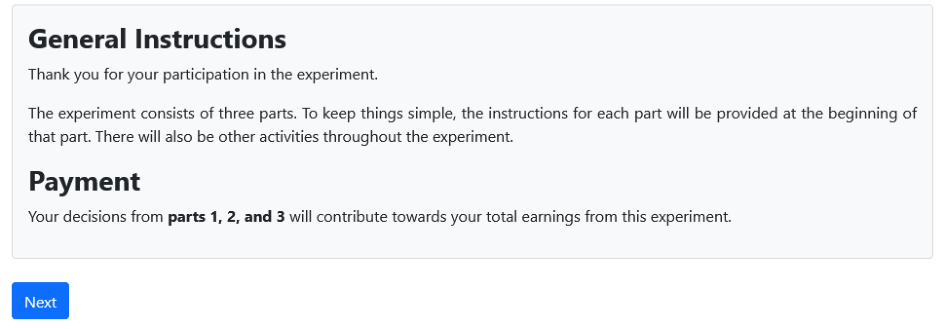
\includegraphics[width=16cm, height=6cm]{General_Screenshot1}
\end{center}

\subsection{Task 1 - Lie}
\begin{center}
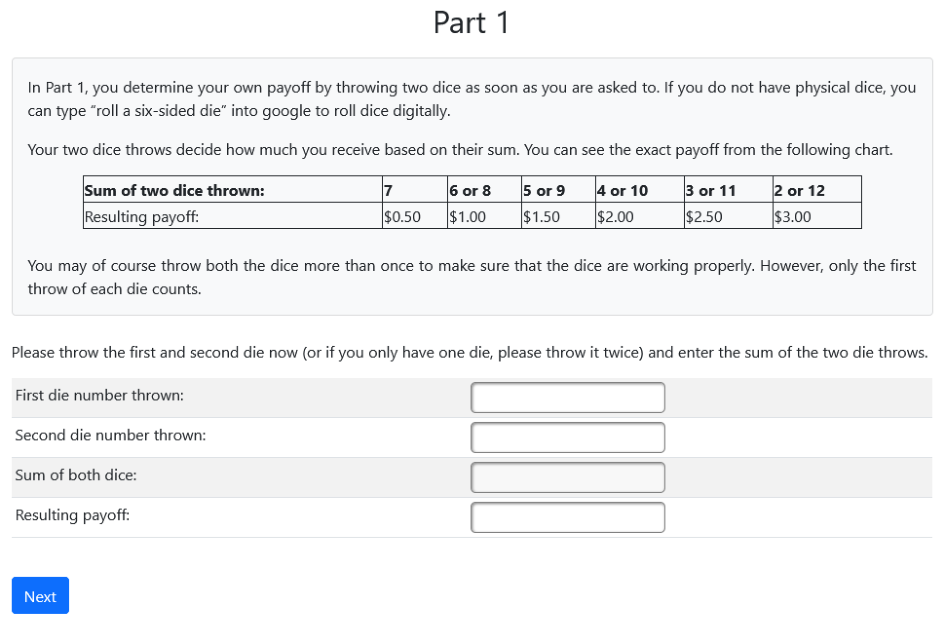
\includegraphics[width=16cm, height=10.5cm]{Lie_Screenshot1}
\\
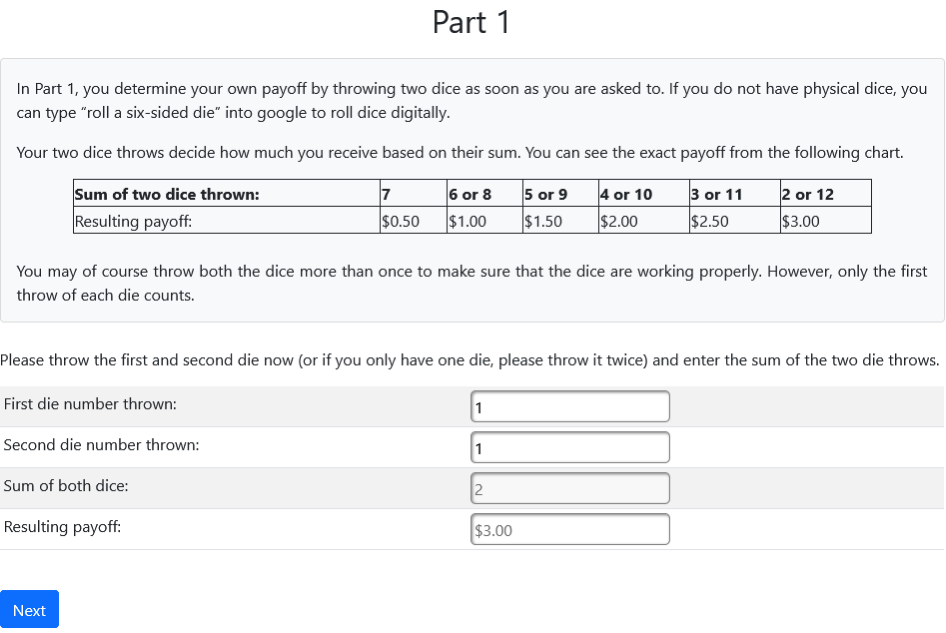
\includegraphics[width=16cm, height=11cm]{Lie_Screenshot2}
\end{center}

\subsection{Task 1 - Luck}
\begin{center}
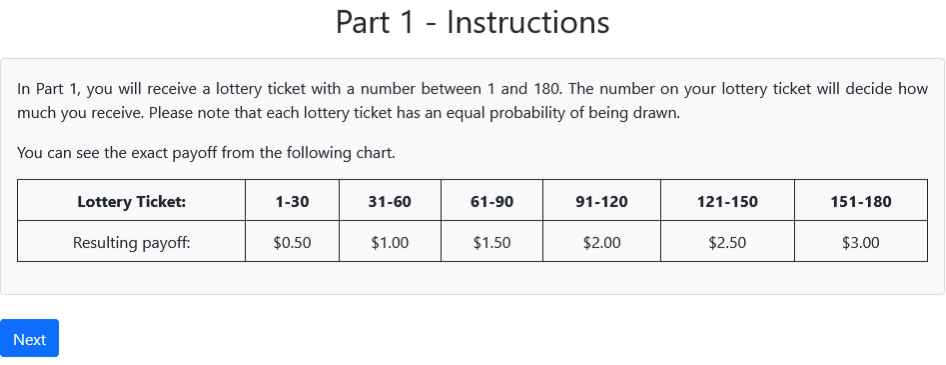
\includegraphics[width=16cm, height=6cm]{Luck_Screenshot1}
\\
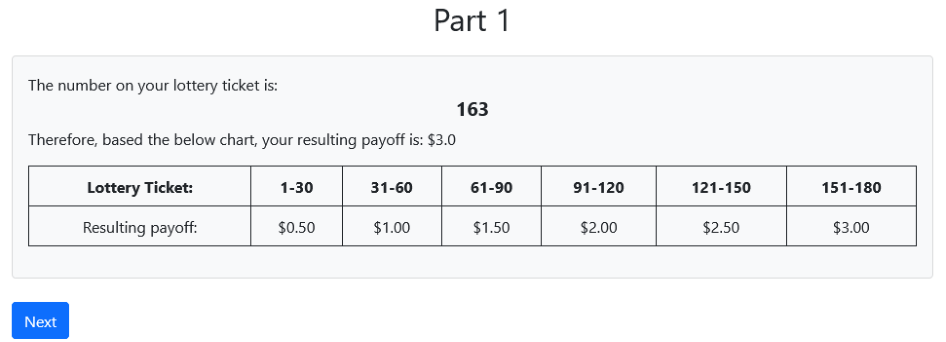
\includegraphics[width=16cm, height=6cm]{Luck_Screenshot2}
\end{center}

\subsection{Task 1 - Base}
\begin{center}
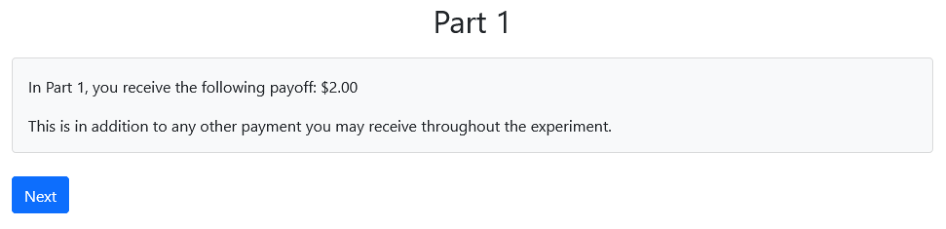
\includegraphics[width=16cm, height=4cm]{Base_Screenshot1}
\end{center}

\subsection{Task 2 - Taking}
\begin{center}
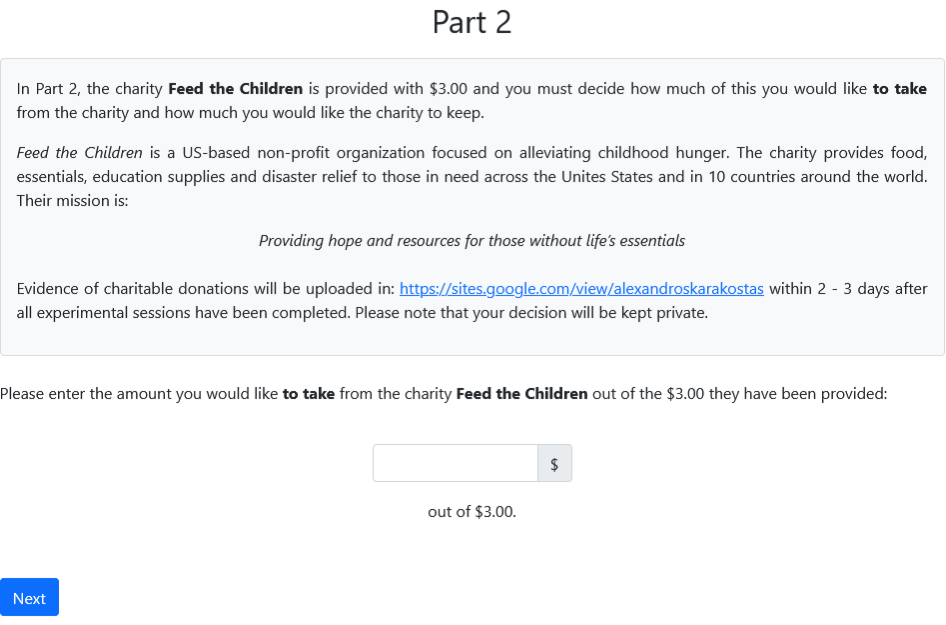
\includegraphics[width=16cm, height=9cm]{Antisocial_Screenshot1}
\end{center}

\subsection{Task 2 - Giving}
\begin{center}
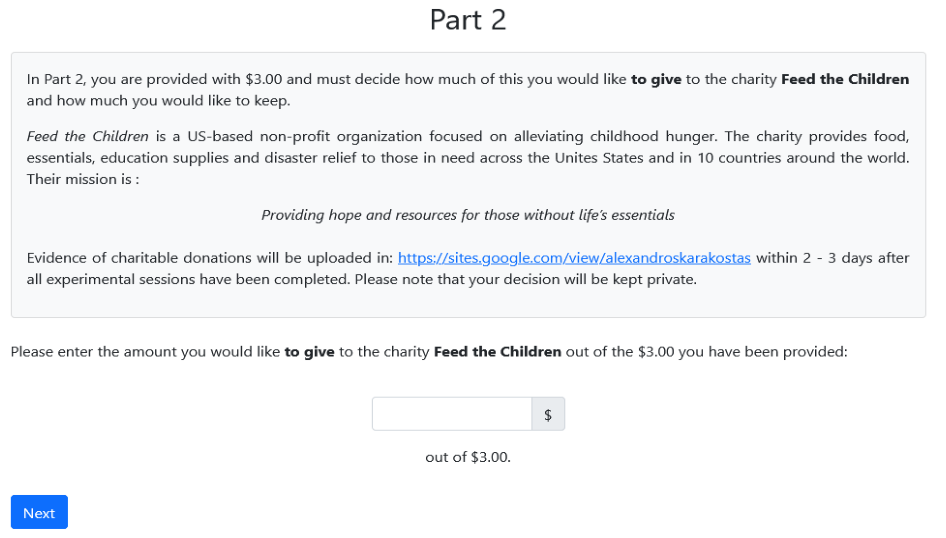
\includegraphics[width=16cm, height=9cm]{Prosocial_Screenshot1}
\end{center}

\subsection{Social Norms Elicitation}
\begin{center}
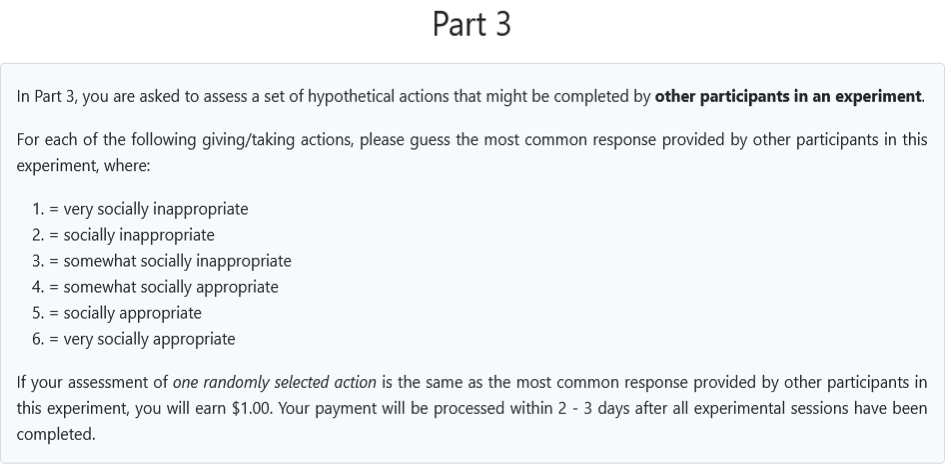
\includegraphics[width=16cm, height=8cm]{SN_Screenshot1}
\\
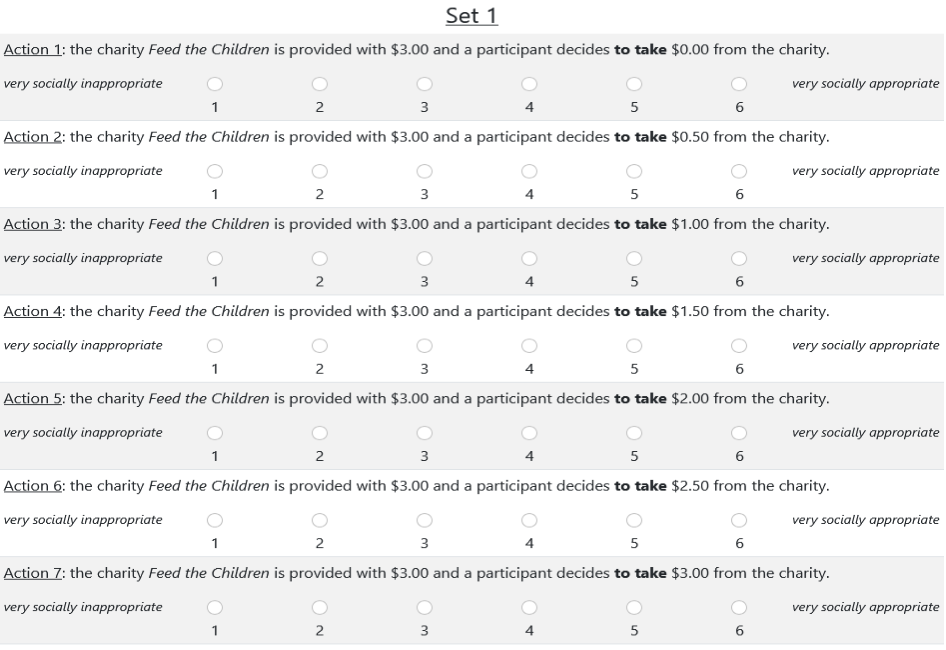
\includegraphics[width=16cm, height=11cm]{SN_Screenshot2}
\\
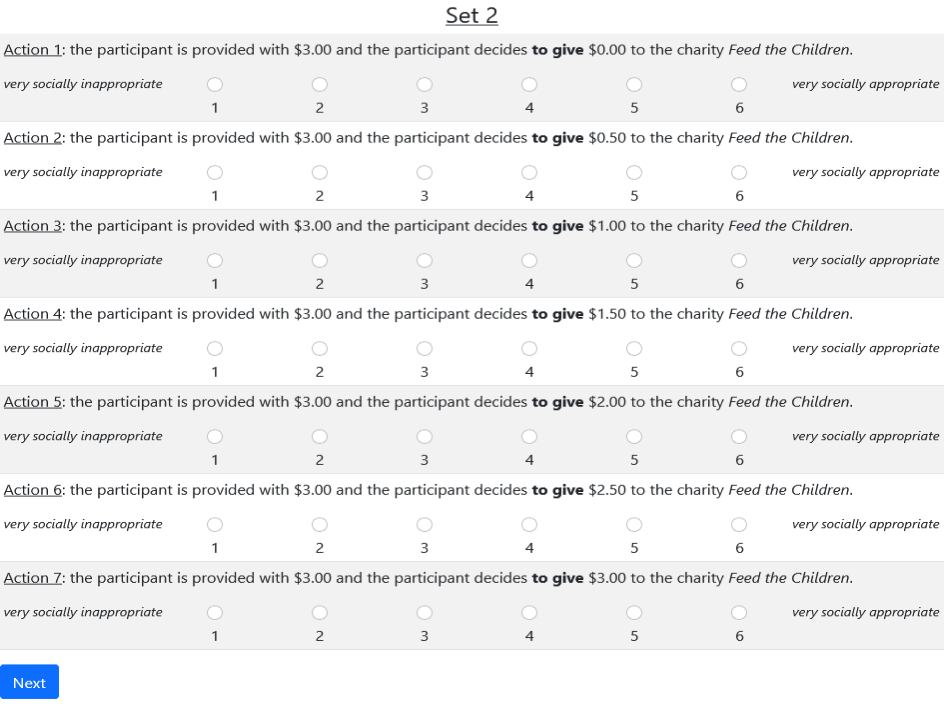
\includegraphics[width=16cm, height=12cm]{SN_Screenshot3}
\end{center}


\subsection{End of Experiment Activities}
\begin{center}
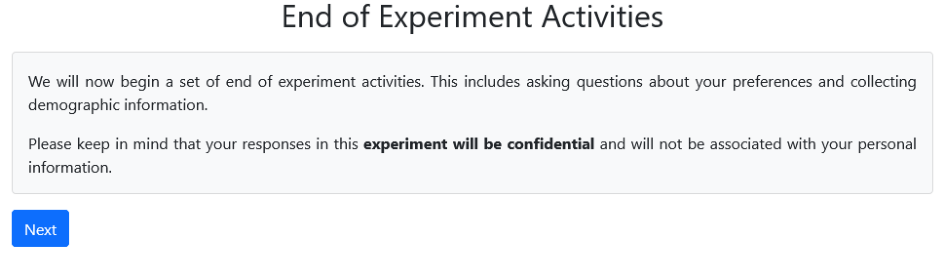
\includegraphics[width=16cm, height=4.5cm]{End_Screenshot1}
\\
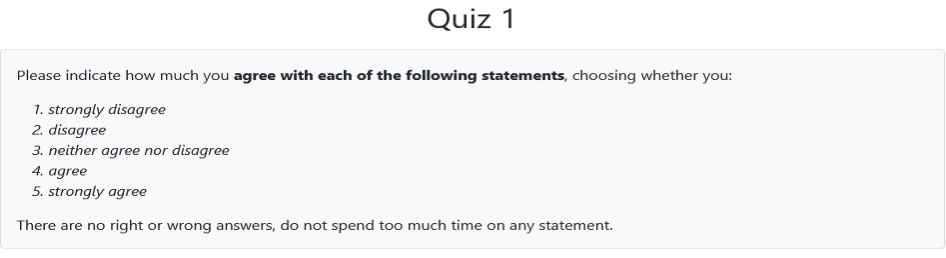
\includegraphics[width=16cm, height=4.5cm]{End_Screenshot2}
\\
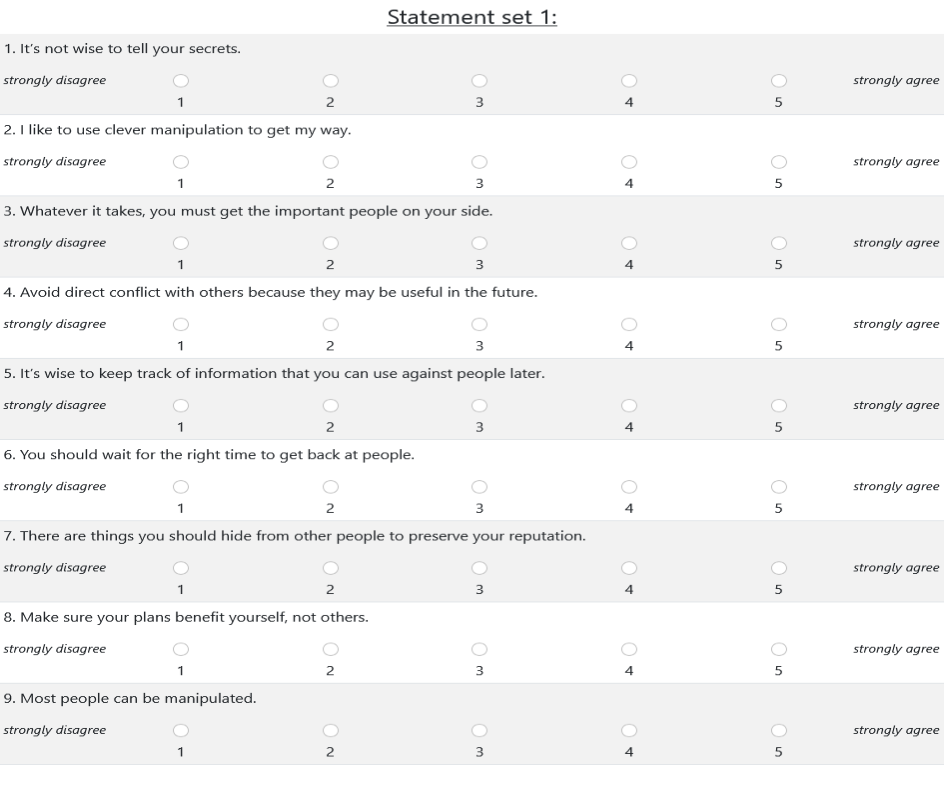
\includegraphics[width=16cm, height=13.5cm]{End_Screenshot3}
\\
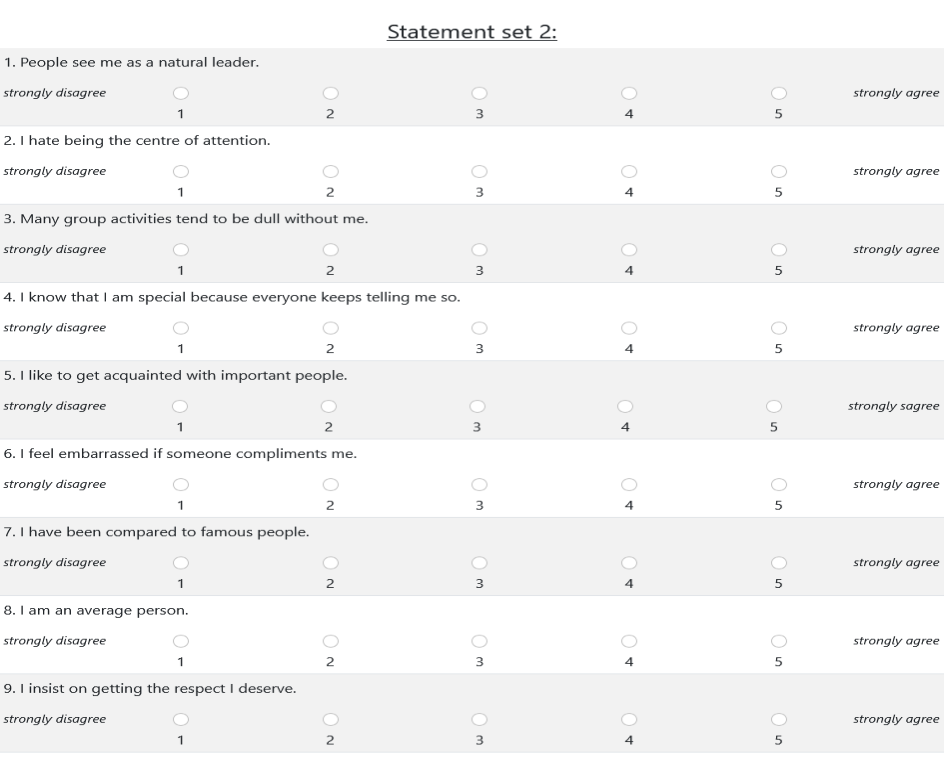
\includegraphics[width=16cm, height=13.5cm]{End_Screenshot4}
\\
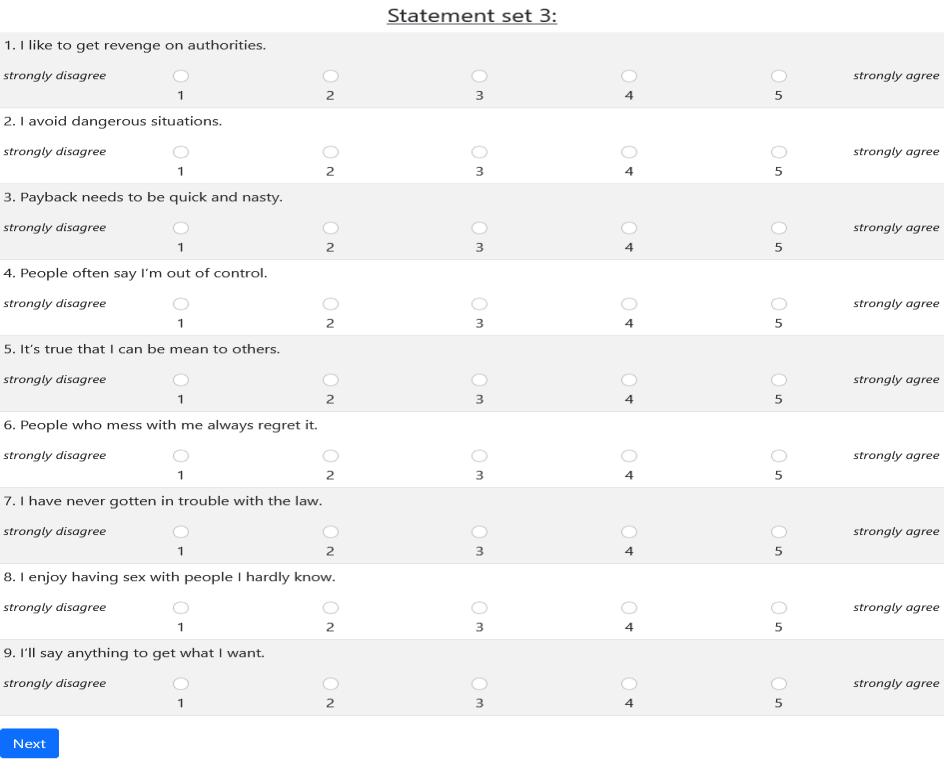
\includegraphics[width=16cm, height=13cm]{End_Screenshot5}
\\
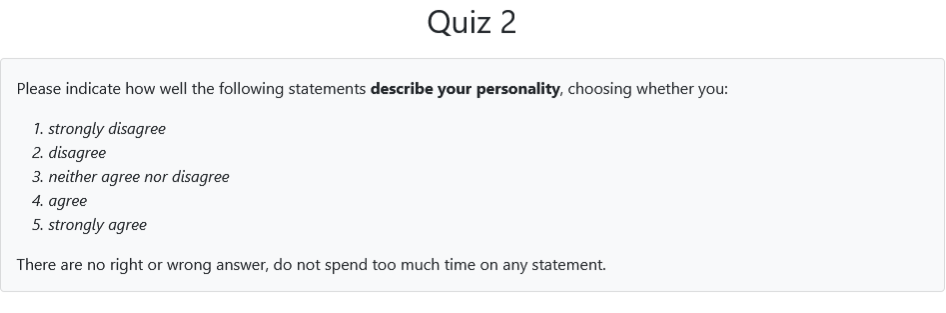
\includegraphics[width=16cm, height=5.5cm]{End_Screenshot6}
\\
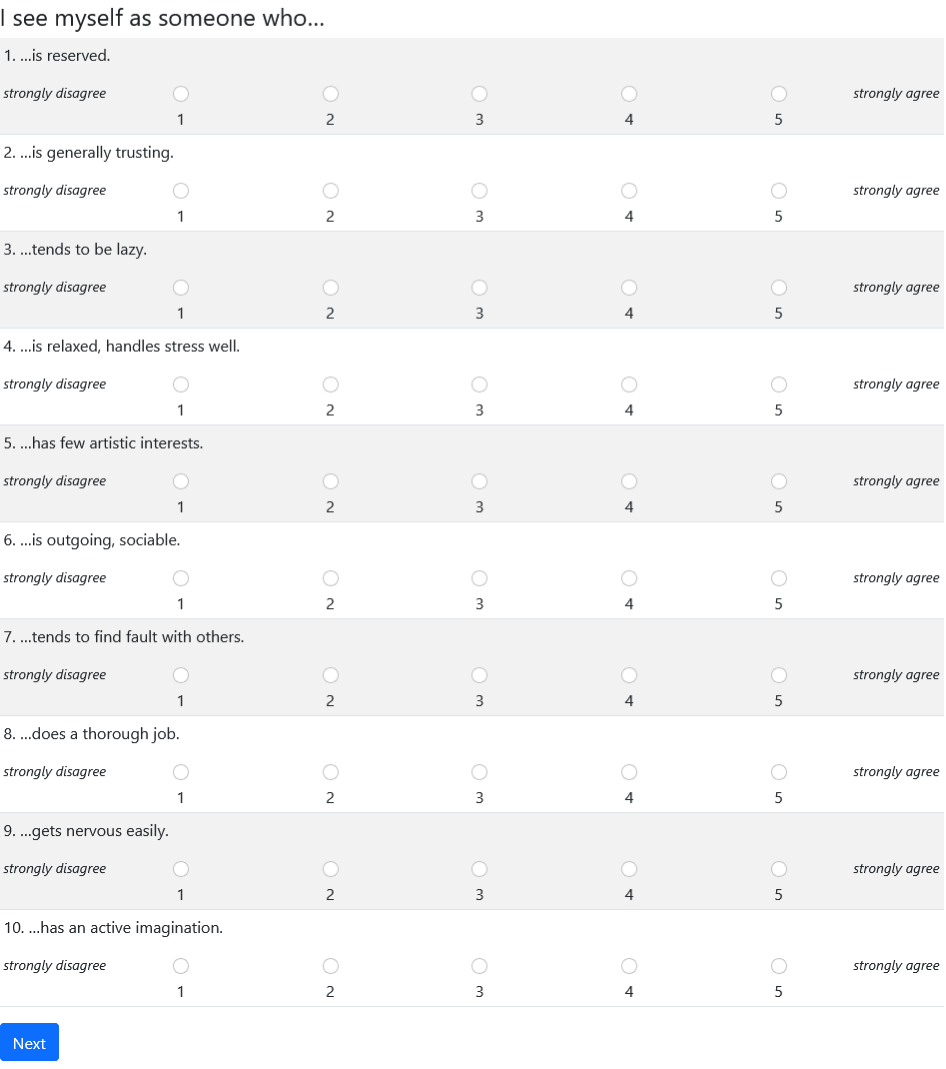
\includegraphics[width=16cm, height=18cm]{End_Screenshot7}
\\
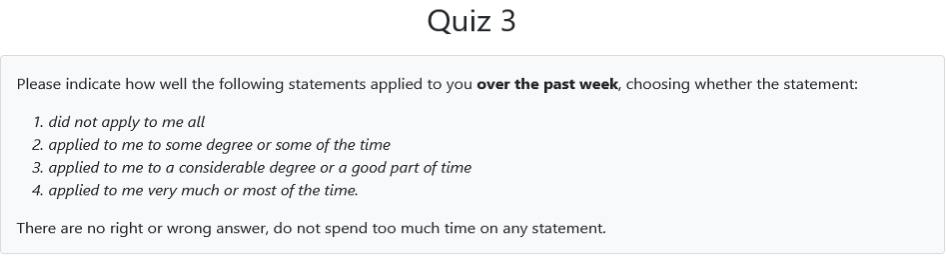
\includegraphics[width=16cm, height=4.5cm]{End_Screenshot8}
\\
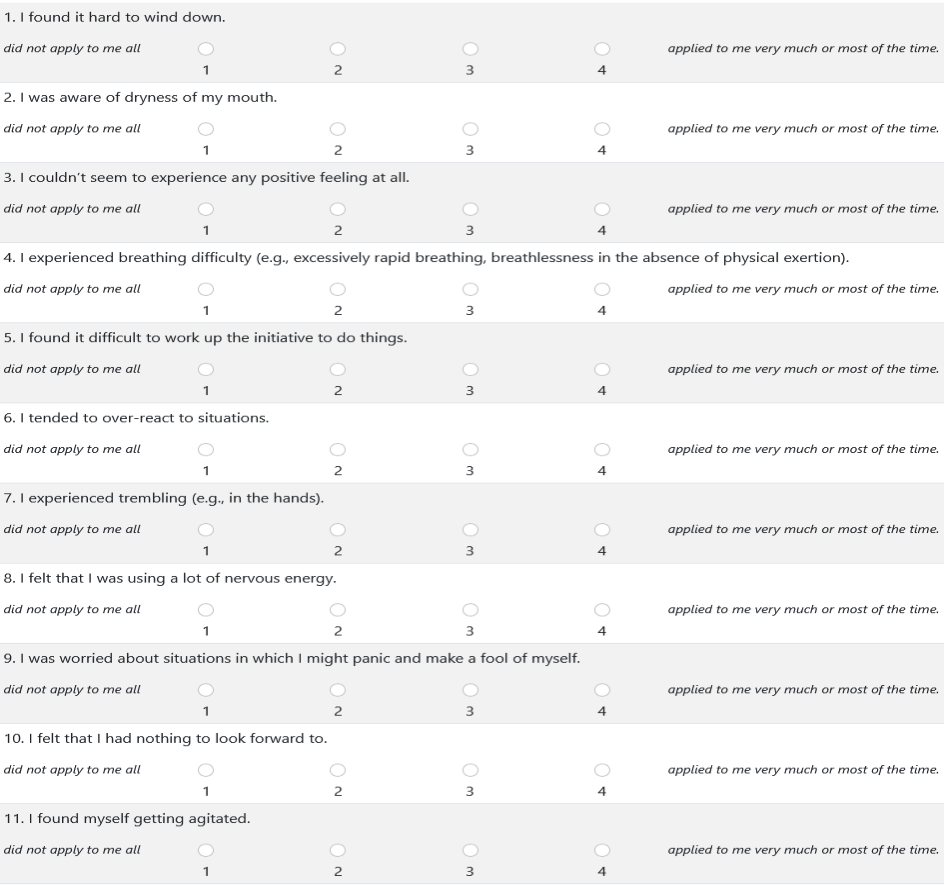
\includegraphics[width=16cm, height=15.5cm]{End_Screenshot9}
\\
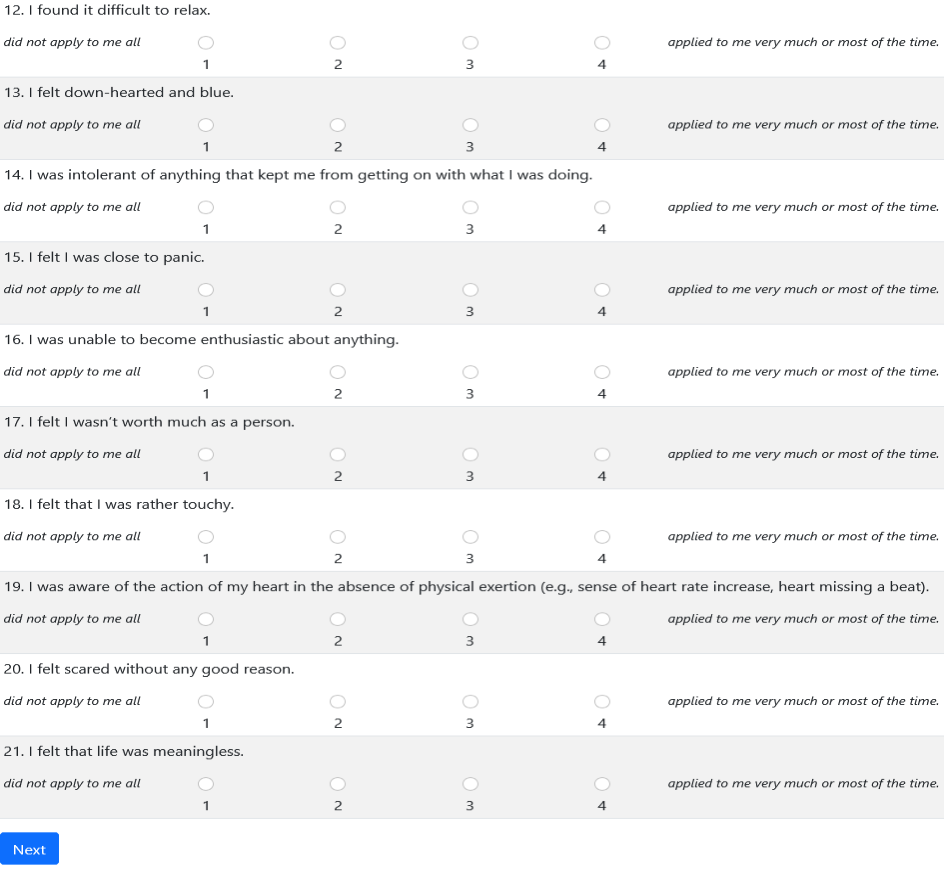
\includegraphics[width=16cm, height=15.5cm]{End_Screenshot10}
\\
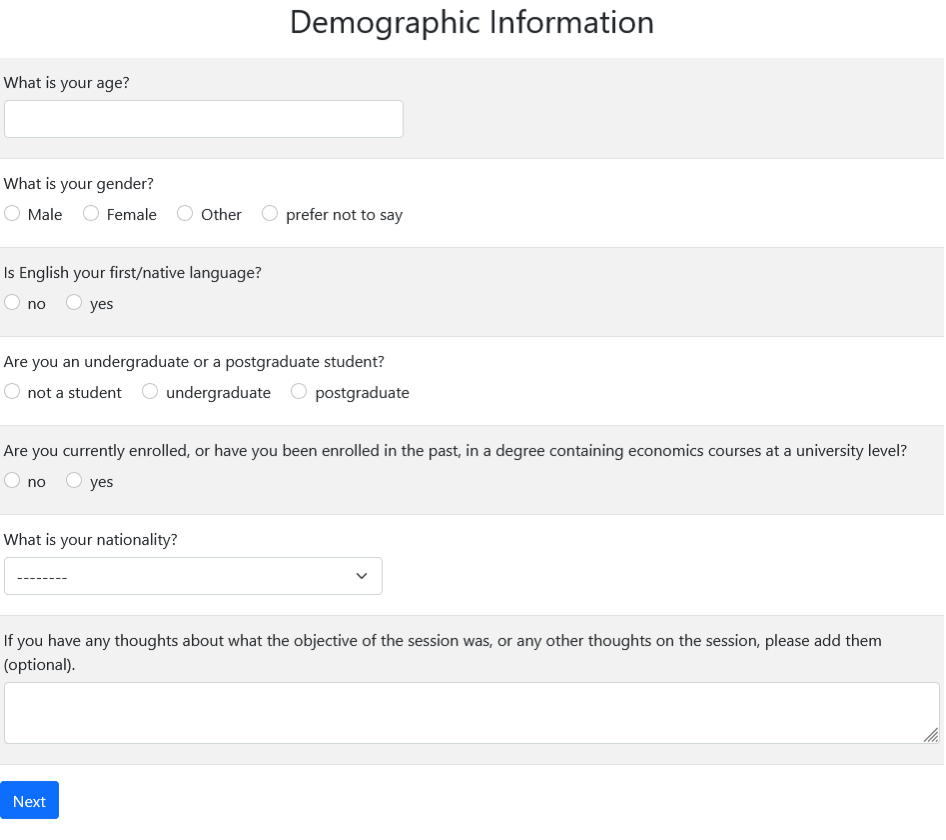
\includegraphics[width=16cm, height=14.5cm]{End_Screenshot11}
\\
\end{center}

\end{document}
